\documentclass[aip, jcp, reprint, onecolumn, nofootinbib]{revtex4-2}

\bibliographystyle{apsrev4-2}

\usepackage{physics}
\usepackage{amsmath}
\usepackage{amssymb}
\usepackage{mathtools}
\usepackage{graphicx}
\usepackage{dcolumn}
\usepackage{bm}
%\usepackage{times}
\usepackage{etoolbox}
\usepackage[colorlinks=true, linkcolor=black, urlcolor=blue, citecolor=black, anchorcolor=black]{hyperref}

\usepackage{lineno}
\linenumbers


\graphicspath{{"figures/"}}
\begin{document}
%Title of paper
\title{Coherent IR-Hyper-Raman Four Wave Mixing Spectroscopy}


\author{Ryan P. McDonnell} %\email{rpmcdonnell@wisc.edu}
\author{Daniel D. Kohler}
\author{John C. Wright} \email{wright@chem.wisc.edu}

\affiliation{Department of Chemistry, 
        University of Wisconsin - Madison, 
        Madison, Wisconsin 53706, 
        United States of America}

\date{\today}

\begin{abstract}
Nonlinear, four wave mixing vibrational spectroscopies are commonly used to probe electron-vibration coupling in isotropic media.
Most of these methods rely on infrared and/or Raman transitions, but methods involving hyper-Raman transitions are also possible. 
Hyper Difference Frequency Generation (HDFG) spectroscopy is an underdeveloped four wave mixing vibrational spectroscopy based upon both infrared absorption and hyper-Raman scattering transitions. 
Despite several experimental reports on HDFG, its spectroscopic properties have not been fully explored. 
To this end, we investigate the selection rules and behavior of HDFG spectroscopy as an upconverted infrared spectroscopy and as a probe of vibronic coupling in molecular systems.
We discuss the similarities between HDFG, a four wave mixing technique, and vibrational sum frequency generation (vSFG) spectroscopy, a three wave mixing technique. 
vSFG and HDFG appear to provide similar output intensities, making HDFG feasible for vSFG practitioners.
HDFG is shown to a sensitive probe of vibronic coupling in bulk systems and provides an alternative method to investigate electronic-nuclear coordinate correlations.
\end{abstract}

\maketitle

\section{Introduction}
Coherent multidimensional spectroscopy (CMDS) is a family of nonlinear spectroscopy methods that form the optical analogue of multidimensional nuclear magnetic resonance (NMR) spectroscopy.\cite{Cho2008}
Multiresonant, four wave mixing CMDS experiments, first proposed by Oudar and Shen in 1980,\cite{RN307} directly probe coupling and correlations between different vibrational, electronic, and vibronic states. \cite{RN281, RN103, Cho2008} 
Four wave mixing CMDS has resolved anharmonicities, ultrafast dynamics, and other inter- and intra-molecular couplings in numerous systems. \cite{Cho2008, Gaynor2017, Ziegler2018, Ogilvie2019, Bonn2021, RN325, Chen2024}
To target vibrational and electronic coupling, methods commonly make use of Raman transitions, e.g., doubly vibrationally enhanced spectroscopy (DOVE), triple sum frequency (TSF), coherent anti-Stokes Raman spectroscopy (CARS), and resonant impulse stimulated Raman spectroscopy (RISRS).\cite{RN103, Dhar1994, RN345, Cho2000, RN491}
Here we explore the less-utilized hyper-Raman transition in four wave mixing CMDS.

\begin{figure*}[!htbp]
	\centering
	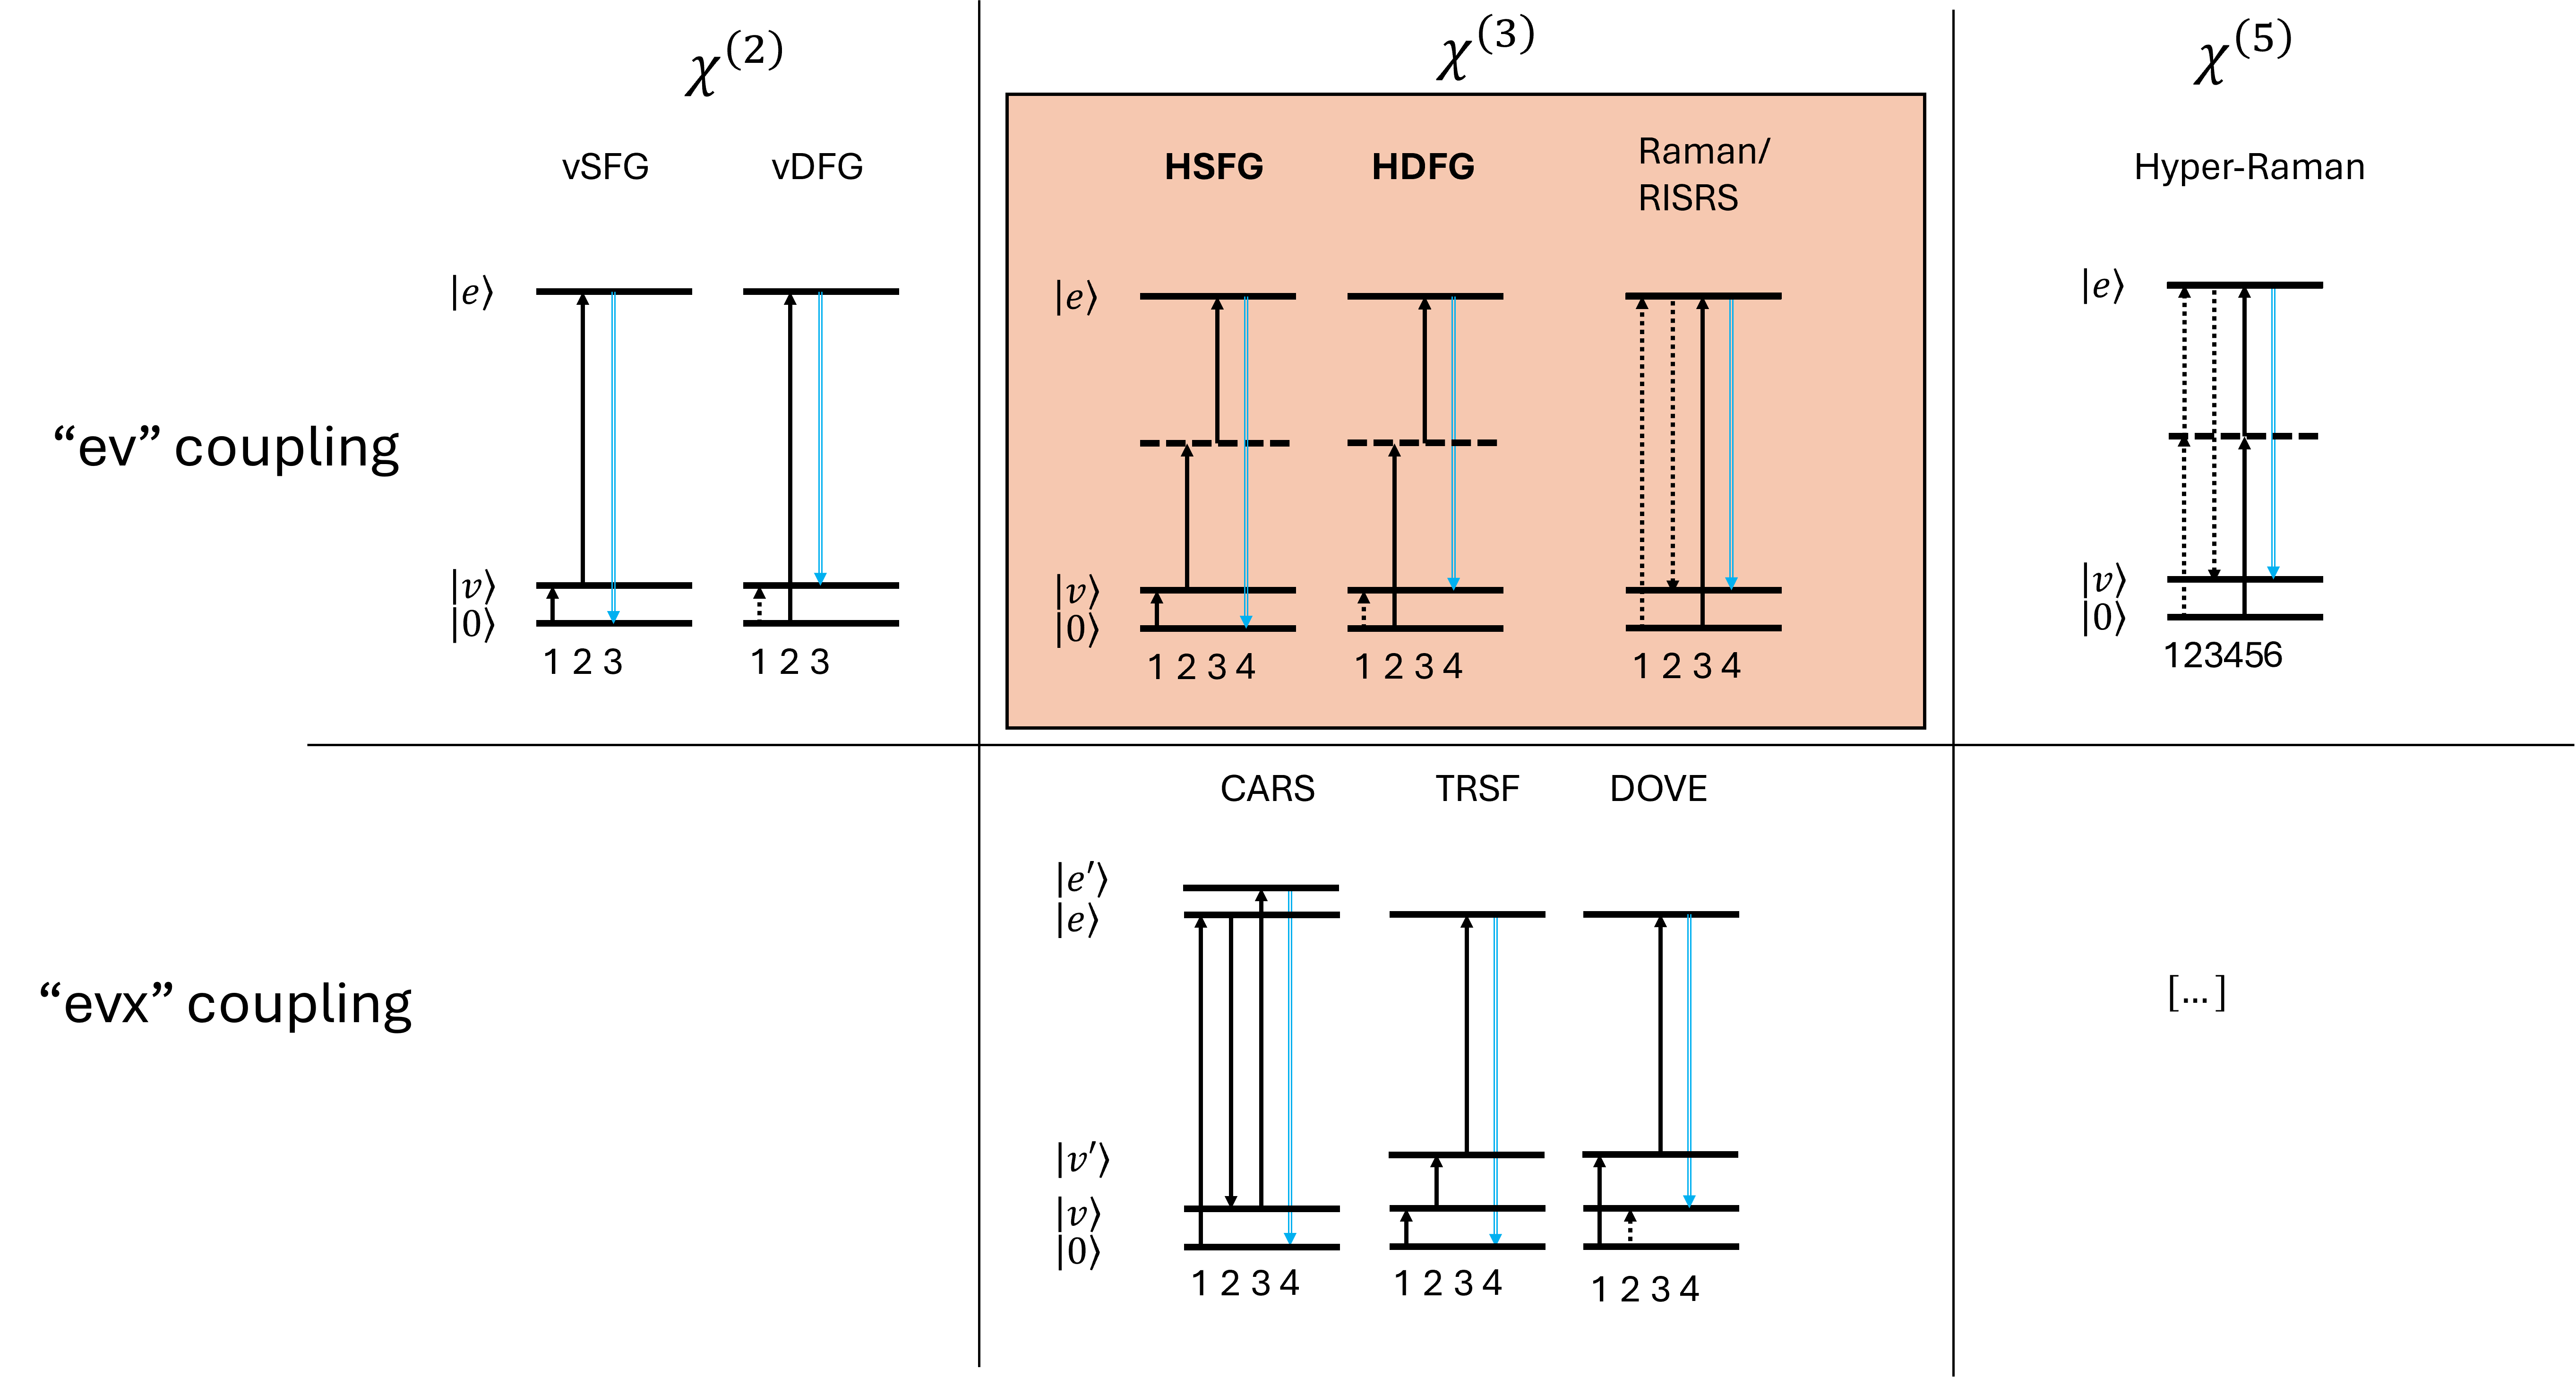
\includegraphics[width=6.66in]{taxonomy.png}
	\caption{
		Some spectroscopic methods for investigating (top) electronic-vibrational coupling and (bottom) e-v-x (x: e, v, e-v, e-v-e) coupling through different order nonlinear processes.
		The light-matter interactions are depicted using Wave Mixing Energy Level (WMEL) diagrams.\cite{RN286}
		Solid and dashed horizontal lines indicate real and virtual states, whereas solid and dotted arrows indicate ket and bra side transitions, respectively. 
		The red box outlines the e-v coupling techniques (HDFG, HSFG) relevant to this manuscript.
	} 
	\label{fig:comparisonwmel}
\end{figure*}

The hyper-Raman transition is the nonlinear, two photon analogue to the Raman transition.\cite{Terhune1965, Cyvin1965, Andrews1978}
Two photons of frequency $\omega_a$ and $\omega_b$ inelastically scatter with matter, promoting or demoting a vibrational mode of frequency $\omega_v$ and emitting a single photon of frequency $\omega_a + \omega_b \mp \omega_v$. 
While most hyper-Raman experiments are performed using degenerate input pulses ($\omega_a = \omega_b$),\cite{RN515} it is possible to perform the technique with non-degenerate input pulses ($\omega_a \neq \omega_b$). \cite{Denisov1986, Kozich2007}
The single photon emission is a significantly different frequency from the excitation frequencies, making rejection of excitation scatter much easier.
Unlike Raman, all infrared active modes are hyper-Raman active, which allows infrared active modes to be probed through a two-photon inelastic scattering event. \cite{Andrews1978}
One drawback is that hyper-Raman transitions are typically weak compared to their Raman counterparts, even when accounting for the high intensities available to ultrafast pulsed lasers.\cite{RN515, Kelley2010}
CMDS methods partially mitigate this issue because emission is spatially coherent so that all emission is directional and easily collected.
In fact, hyper-Raman transitions have been observed in several CMDS studies (sometimes under the moniker of SIVE, or singly vibrationall enhanced spectroscopy).\cite{Zilian1994, RN350, RN351, RN352, RN353, Chen1998, RN362, RN418, Hanninen2018, Wang2021, Bonn2024, McDonnell2024}

Hyper difference frequency generation (HDFG) spectroscopy and hyper sum frequency generation (HSFG) spectroscopy are four wave mixing CMDS methods based on direct excitation of a vibrational mode through IR absorption and subsequent scattering to or from the vibrational mode through a hyper-Raman transition.
In HDFG/HSFG, an infrared pulse is resonant with a vibrational mode, while two other excitations stimulate the hyper-Raman process.
The infrared excitation frequency selects the vibrational mode stimulated through the hyper-Raman transition.
The other two excitation frequencies control electronic enhancement for the hyper-Raman scattering event.

The HDFG and HSFG processes and related spectroscopies that investigate vibrational-electronic coupling are diagrammed in \autoref{fig:comparisonwmel} using Wave Mixing Energy Level (WMEL) diagrams. \cite{RN286}
The three-wave mixing ($\chi^{(2)}$) techniques are often less applicable as they require macroscopic non-centrosymmetry under the electric dipole approximation.\cite{RN480}
Hyper-Raman scattering itself is a six-wave mixing ($\chi^{(5)}$) technique; stimulated hyper-Raman will be weak and susceptible to four-wave mixing (FWM) cascades.\cite{RN515, RN243, Cho2000_Cascade}
A coherent six-wave mixing analogue of hyper-Raman scattering, coherent anti-Stokes hyper-Raman spectroscopy (CAHRS), has been proposed and explored theoretically by several authors; however, it is also weak and susceptible to FWM cascades.\cite{Taran1977, Berger1978, Bjarnason1980, Cho1997, Cho1998}
Of the many four-wave mixing techniques, HDFG and HSFG have strong similarity to Raman, stimulated Raman, and RISRS in that the electronic state must remove or add a $v$ quantum to the ground state (``ev'' coupling).
With the other four-wave and six-wave mixing techniques (\autoref{fig:comparisonwmel}, second row), the output signal depends on more states than just a single vibrational mode and electronic state (``evx'' coupling).\cite{RN445, RN335} 
As a result, the relationship between the output and vibrational-electronic coupling is more detailed, but also more complicated.
HDFG, HSFG and Raman are more direct probes of electronic-vibrational coupling.
Notably, HDFG and HSFG can be implemented as two-color experiments (with $\omega_2=\omega_3$);\cite{Cho2001} vibrational sum frequency generation (vSFG) or difference frequency generation (vDFG) setups can be trivially reconfigured to perform HSFG or HDFG measurements to investigate ev coupling in bulk systems.

Nonlinear spectroscopic probes of electronic-vibrational coupling are not limited to the Raman and hyper-Raman based techniques diagrammed in \autoref{fig:comparisonwmel}.
Independently developed by the Fleming and Khalil groups, respectively, 2D Electronic-Vibrational (2D-EV) and 2D Vibrational-Electronic (2D-VE) spectroscopy are $\chi^{(3)}$ methods based upon pump-probe and absorption type pathways which also investigate e-v coupling.\cite{Oliver2014, Courtney2015, Courtney2015_1}
The Rao group has also developed 2D-EV sum frequency generation (2D-EVSFG), a $\chi^{(4)}$ analogue of 2D-EV, to probe interfacial e-v coupling. \cite{Deng2021}  
These methods have been used to understand vibronic coupling in a variety of molecular systems and, albeit with different selection rules, serve as 2D pump-probe type analogues to the infrared-hyper-Raman spectroscopies discussed here.

When the hyper-Raman excitation in HDFG or HSFG is resonant or near-resonant with electronic states, the brightness of the vibrational feature depends on the vibronic structure of the electronic state.
The electronic spectrum probed in HDFG or HSFG can inform on processes that control ultrafast electronic relaxation in molecular and biological systems in ways similar to resonance Raman.\cite{Cho2001, Bredenbeck2015, Gaynor2018, Arsenault2021}
Since the selection rules of hyper-Raman scattering differ from Raman scattering, the hyper-Raman excitation spectra give a unique alternative to Raman scattering to understand vibrational spectra, electronic structure and vibronic coupling in molecular systems. \cite{Olson2018}

This paper investigates the microscopic parameters that control HDFG output. \cite{RN352, Bonn2024, McDonnell2024}
HSFG will not be discussed, but the application of our treatment to HSFG is straightforward and the results are similar.
We note that HDFG emission can be phase-matched in media with normal dispersion while HSFG cannot.\cite{RN279, RN278} 
This paper is organized as follows.
In \autoref{steadystate}, we first identify the HDFG vibrational selection rules. 
The electronically-resonant HDFG selection rules are then identified through an expansion of electronic dipole moments following Chung and Ziegler.\cite{Ziegler1988}
HDFG is found to be allowed in any harmonic system that has infrared active vibrations.
A simple harmonic oscillator model system is used to simulate HDFG spectra and illustrate how the excited state potential energy surface affects the hyper-Raman excitation spectrum.
After developing selection rules, some quantitative aspects of HDFG are discussed in \autoref{quant}.

\section{Selection Rules for HDFG Spectroscopy}\label{steadystate}

In this section, we investigate the properties of HDFG and make the connections between HDFG and hyper-Raman scattering explicit.
Coherent spectroscopies are often described using the density matrix formalism in the interaction picture, where an n$^{\text{th}}$ order density matrix $\rho^{(n)}$ is propagated using the Liouville-von Neumann equation:
\begin{equation}\label{LVNE}
	\dot{\rho}^{(n)} = \frac{1}{i \hbar} [H + V(t), \rho^{(n-1)}] + \dot{\rho}^{(n)}_R,
\end{equation}
where $H$ is the (static) system Hamiltonian, $V(t)$ is the field-matter interaction and $\rho_R$ is the relaxation density matrix. \cite{RN455}
In systems where interactions with surroundings are relevant, expressions for $\dot{\rho}_R$ may be quite complicated due to intricate phenomena such as system-bath interactions and solvent-solute coupling, among others. \cite{Sung2001}
In the limit where input field pulse widths are much longer than electronic dephasing times and the individual molecule limit is approached, it becomes acceptable to write a time-independent relaxation matrix $\dot{\rho}^{(n)}_R= \Gamma \rho^{(n)}$, i.e., exponential relaxation, where $\Gamma$ is the system's dephasing rate. \cite{RN455, Sue1986, Sung2001}
While exponential relaxation is usually an inappropriate description of most physical systems involving solvent-solute interactions,\cite{Sue1986, Yan1988, Li1994, Myers1997} our goal is to introduce simple, qualitative models to understand HDFG response.
Thus, we write $\dot{\rho}^{(n)}_R= \Gamma \rho^{(n)}$.
The exponential relaxation limit has proven useful in investigating the properties of 2D-EV, 2D-VE, and doubly resonant SFG using pulses much longer than electronic dephasing times. \cite{Raschke2002, Gaynor2017}

It is useful to briefly discuss the impact of time ordering on HDFG output.
Dependent upon the time-ordering schemes, it is possible to eliminate output through destructive interference.\cite{Cho2008}
While we have only isolated one specific HDFG resonance and time-ordering scheme (\autoref{fig:comparisonwmel}), there are several other pathways which can provide HDFG output. \cite{RN352}
If $\omega_2$ becomes resonant and $\omega_1$ becomes non-resonant, where $\omega_2 > \omega_1$, then other HDFG pathways appear (\autoref{fig:sivewmel2}c-f).\cite{McDonnell2024} 
While the methods in \autoref{fig:sivewmel2} possess identical selection rules to \autoref{fig:comparisonwmel}, the pathways presented in \autoref{fig:sivewmel2} will interfere, which can amplify or decrease coherent output.
\begin{figure*}[!htbp]
	\centering
	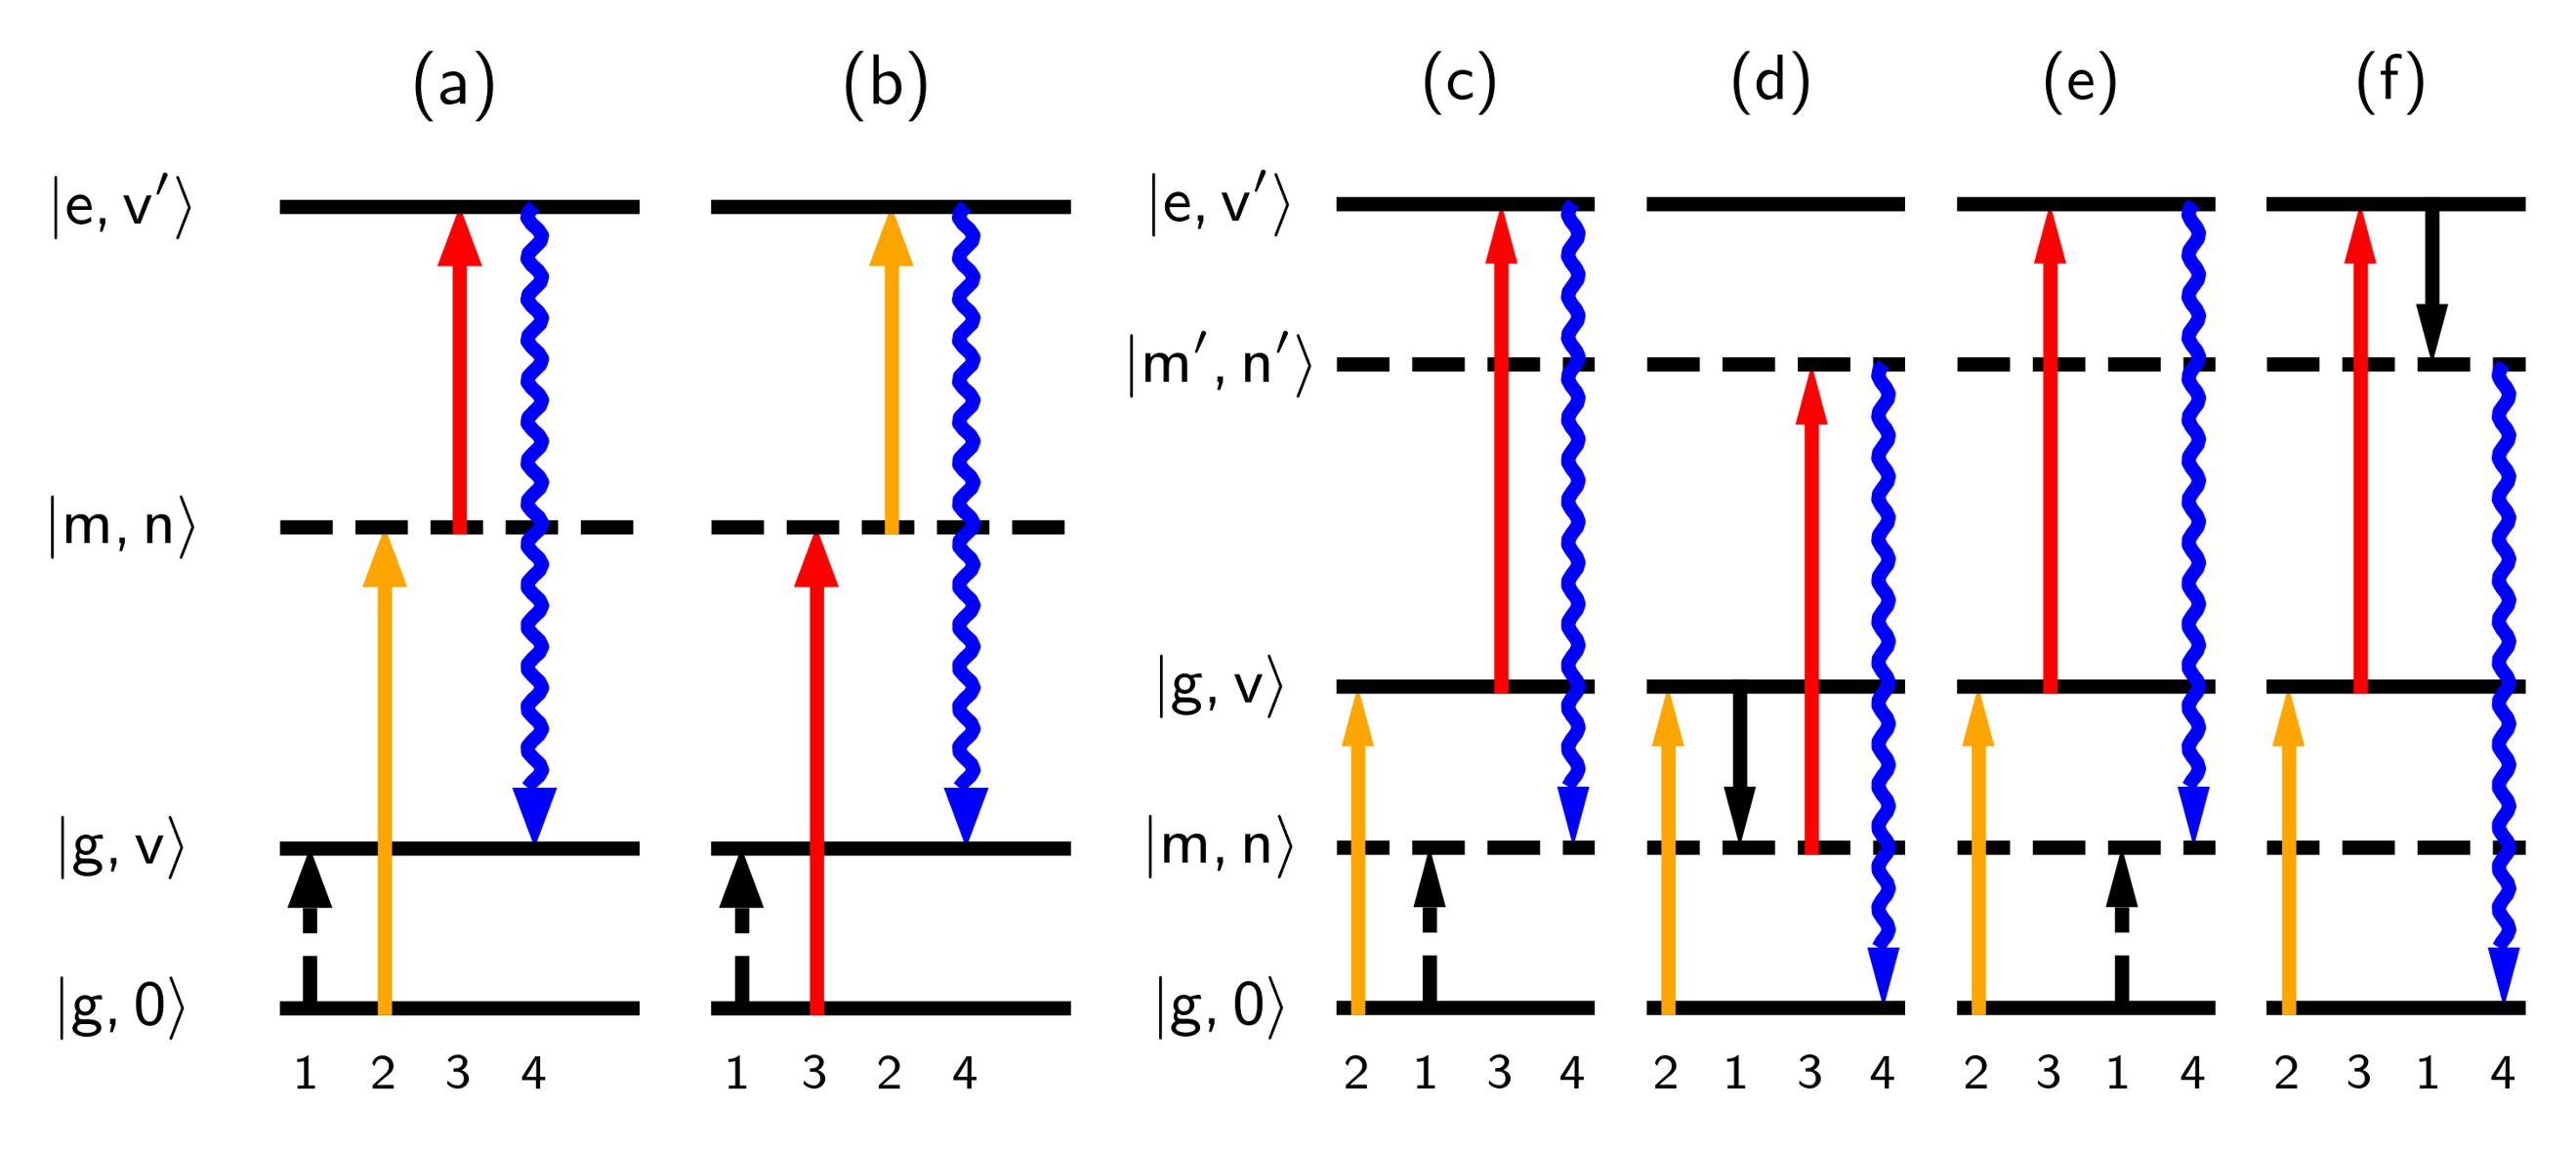
\includegraphics[width=\textwidth]{figures/timeorderedwmel.png}
	\caption{WMEL diagrams of HDFG pathways for when (a,b) $\omega_1$ (black arrow) interacts first and (c-f) $\omega_2$ (orange arrow) interacts first. 
		In (a,b), $\omega_1$ is resonant with a vibrational mode, but in (c-f), $\omega_2$ is resonant with a vibrational mode.
		The states are labeled as $\ket{a,b}$, where $a$ refers to an electronic state and $b$ refers to quanta in a vibration on $a$, described in \autoref{Albrecht}.
		In all cases, $\omega_2 > \omega_1$.
	}
	\label{fig:sivewmel2}
\end{figure*}

In the limit where $\omega_2+\omega_3$ is detuned from an electronic resonance, it becomes simple to interpret the interference schemes. 
The case where $\omega_1$ interacts first and is resonant, and $\omega_2 + \omega_3$ is nonresonant, yields two contributed pathways: \autoref{fig:sivewmel2} (a) and (b).
These pathways possess identical phase and transition moments, which yields total constructive interference, assuming similar non-resonant dispersion from each pathway.
Conversely, in the case where only $\omega_2$ is resonant, diagrams (c,d) and (e,f), when detuned from an electronic resonance, have identical transition moments but opposite phase. 
As a result, the output from (c,d) and (e,f) completely destructively interfere; no signal can be obtained from these pathways when significantly detuned from an electronic state. \cite{McDonnell2024}
Note that in the case where $\omega_1$ interacts first but only $\omega_2$ is resonant, the nonlinear output generated nearly vanishes as the first resonant pulse arrives after a non-resonant pulse.

When $\omega_2 + \omega_3$ becomes electronically resonant, the interference changes for the \autoref{fig:sivewmel2}c-f pathways.
Note that in this regime, only pathways (c,e,f) possess identical transition moments.
As a result, pathways (c,d) survive and can provide output when $\omega_2+\omega_3$ is resonant with an electronic state. 
These results provide a simple rule of thumb for collecting HDFG spectra: use \autoref{fig:sivewmel2}a,b pathways to measure spectra when significantly detuned from an electronic resonance, and any of these vibrationally resonant pathways can measure spectra when electronically resonant.
However, since electronic states commonly have short dephasing times and significant inhomogeneous broadening,\cite{Dong2015, Lewis2015} it is likely the \autoref{fig:sivewmel2}f pathway will become triply resonant and possibly contribute greater than the other pathways. 
Such instances are system dependent. 
Discussion will be isolated to the \autoref{fig:sivewmel2}a pathway in the sections that follow.

Other potential interferants in HDFG spectroscopy are direct and sequential cascades of second-order vDFG and vSFG processes.\cite{RN297, Cho2000_Cascade, RN301}
While unimportant in achiral isotropic systems,\cite{Belkin2000} second-order cascades may become important in media where SFG and DFG are allowed, e.g. chiral media, interfaces or non-centrosymmetric media. 
Nevertheless, in the discussion that follows for the rest of this manuscript, we will assume isotropic media, and therefore negligible second-order cascades. 

It is useful to expose relationships between nonlinear output, transition dipoles and hyper-Raman hyperpolarizabilities in the driven limit ($\dot{\rho}^{(n)} = 0 \ \forall n$). \cite{Moad2005}
Under the electric dipole approximation, the $I^\text{th}$ Cartesian component of the third order nonlinear output polarization, ${P}^{(3)}_I$, of a four wave mixing process, induced by electric fields $E_J$, $E_K$, and $E_L$ at output frequency $\omega_4=-\omega_1 + \omega_2 + \omega_3$ is written as (using Einstein summation) \cite{RN307}
\begin{equation} \label{polarization}
{P}^{(3)}_I (\omega_4)  = \varepsilon_0 \chi^{(3)}_{IJKL} E_J(\omega_3) E_K(\omega_2) E_L(- \omega_1) 
\end{equation}
where $\chi^{(3)}_{IJKL}$ is the $IJKL$ element of the third order electrical susceptibility, a rank four tensor, generally written as
\begin{equation}\label{eq:nfgamma}
	\chi^{(3)}_{IJKL} = NF \langle \gamma_{ijkl} \rangle_{IJKL}.
\end{equation}
For clarity, we define the input electric fields as plane waves, where (suppressing the spatial dependence for simplicity)
\begin{equation}
	\vec{E}\left(\omega \right) = \frac{1}{2} \left(\vec{E}_0 \exp\left(i \omega t\right) +\text{c.c.}\right) .
\end{equation}
In \autoref{eq:nfgamma}, $N$ is a number density, $F=\prod_j  \frac{1}{3} \left({\left(n(\omega_j)\right)^2 + 1} \right)$ is the Lorentz local field factor, where $n$ is the (frequency dependent) refractive index and $\gamma_{ijkl}$ is the third-order polarizability (i.e., second hyperpolarizability). \cite{Bedeaux1973}
The brackets indicate an orientational average.\cite{Andrews1977}
Uppercase letters refer to laboratory frame coordinates and lower case letters refer to corresponding molecular frame coordinates.
The steps behind orientational averaging of $\gamma_{ijkl}$, a rank four tensor in the molecular frame, are detailed elsewhere.\cite{Andrews1977, McDonnell2024}

By propagating \autoref{LVNE} in the steady state limit,\cite{Prior1984} the HDFG hyperpolarizability is 
\begin{equation}\label{sivegamma}
		\gamma_{ijkl}^{vg} =	- \sum_{e,m} \frac{1}{\varepsilon_0} \frac{1}{4D} \frac{1}{\hbar^3} \frac{\mu^{ve}_{i} \mu^{em}_{j} \mu^{mg}_{k} \mu^{gv}_{l} }{\Delta_{ev}^{3+2-1} \Delta_{mv}^{2-1}\Delta_{gv}^{-1}}  \rho^{(0)}_{gg}
\end{equation}
where: $\mu^{ab}_{j}$ is the $j^{th}$ element of $\mel{a}{\vec{\mu}}{b}$, $\Delta_{kl}^{-x+y+z} = \omega_{kl} - (-\omega_{x}+\omega_{y} + \omega_{z}) - i\Gamma_{kl}$, $\omega_j$ is the frequency of the j$^{th}$ input field, $\Gamma_{kl}$ is the $\rho_{kl}$ dephasing, and $\rho^{(0)}_{gg}$ is the ground state population.
Here, $\ket{e}$ and $\ket{m}$ are virtual states, and thus necessarily summed over in \autoref{sivegamma}.
The pulse identifiers on the $\Delta_{kl}$ terms will be suppressed henceforth for legibility.
$D$, the Maker-Terhune degeneracy factor, accounts for permutation symmetry of the excitation fields.\cite{RN134} 
For a HDFG experiment using two (three) distinct, non-degenerate input fields, $D = 3 (6)$.

\subsection{Vibrational Selection Rules}

It is useful to investigate the selection rules without vibronic resonance to understand how HDFG can be used as an upconverted infrared spectroscopy.
We first investigate the HDFG selection rules through a Placzek type formalism.
When $\omega_2+\omega_3$ is significantly detuned from resonance and the vibronic nature of the virtual states is ignored, the Placzek approximation can be invoked to study selection rules in terms of the hyper-Raman hyperpolarizability, $\beta$. \cite{Placzek1934, Long1970}
Summing over the virtual states $\ket{e}$ and $\ket{m}$ forms the hyper-Raman hyperpolarizability so that\cite{Long1970} 
\begin{equation}\label{sivebeta}
	\gamma_{ijkl} =	-\frac{1}{\varepsilon_0} \frac{1}{4D \hbar}\frac{\beta^{vg}_{ijk} \mu^{gv}_{l}}{\Delta_{gv}} \rho^{(0)}_{gg}.
\end{equation}
Since all infrared active transitions are hyper-Raman active, HDFG is allowed for any infrared active transition. \cite{Andrews1978}
This selection rule is generally valid for any HDFG or HSFG process when $\omega_2$ and $\omega_3$ are sufficiently detuned from any resonance.

The general selection rule can be simplified by considering the excitation of an infrared active normal mode.  
Assume $\ket{v}$ is the $v^{\text{th}}$ normal mode.
We Taylor expand the dipole and first hyperpolarizability operators to first order in the normal mode coordinate $Q_v$ about equilibrium:
\begin{subequations}
	\begin{equation}
		\mu_l = \mu_{l,0} + \left(\frac{\partial \mu_l}{\partial Q_v}\right)_0 Q_v 
	\end{equation}
	\begin{equation}
		\beta_{ijk} = \beta_{ijk,0} + \left(\frac{\partial \beta_{ijk}}{\partial Q_v}\right)_0 Q_v
	\end{equation}
\end{subequations}
Taking $\ket{g} = \ket{0}, \ket{v} = \ket{1}$, substituting into \autoref{sivebeta} and using typical Harmonic Oscillator selection rules, gives the HDFG hyperpolarizability to $\order{Q_v}$ as \begin{equation}\label{SIVEselection}
	\gamma_{ijkl} =	-\frac{1}{\varepsilon_0} \frac{1}{8D \omega_{vg}}  \frac{1}{{\Delta_{gv}}} \ \left(\frac{\partial \beta^{vg}_{ijk}}{\partial Q_v}\right)_0 \left({\frac{\partial \mu^{gv}_{l}}{\partial Q_v}}\right)_0  \rho^{(0)}_{gg},
\end{equation}
where we have used $\mel{v}{\mu_{l,0}}{g} = 0 = \mel{1}{\beta_{ijk,0}}{0}$, and $\mel{1}{Q_v}{0} = \sqrt{\frac{\hbar}{2\omega_{vg}}}$.
Here, $\omega_{vg}$ is the characteristic $\ket{0} \rightarrow \ket{1}$ frequency.\cite{RN459}
Since \autoref{SIVEselection} is non-zero in the harmonic oscillator limit, HDFG output is allowed for infrared active normal modes in the harmonic limit. 

\subsection{Vibronic Selection Rules}\label{Albrecht}
While the Placzek treatment provides selection rules for vibrationally resonant HDFG output, it does not predict HDFG output as $\omega_2 + \omega_3$ is changed.
We now explicitly consider electronic resonances through the $A,B,C$ decomposition of $\beta$ introduced by Chung and Ziegler, analogous to Albrecht's treatment of Raman spectroscopy (i.e., sum-over-states formalism).\cite{Albrecht1961, Ziegler1988} 
To employ this formalism, we write the states in a Born-Oppenheimer basis $\ket{a,b}$, where $\ket{a,b} = |a(\textbf{Q})) \otimes \ket{b}$ for electronic states $\{|a(\textbf{Q}))\}$ and vibrational states $\{\ket{b}\}$ (i.e., adiabatic approximation), where \textbf{Q}, the system normal modes, is the adiabatic parameter. \cite{BornOppenheimer, Tang1970}
We will henceforth suppress the dependence of the electronic states on \textbf{Q} for simplicity.
It is worthwhile noting that the time-dependent Raman formalism developed by Heller \textit{et al.} can be applied to hyper-Raman scattering. \cite{Lee1979, Shoute2005, Silverstein2012}
However, since our goal is to expose the Quantum Mechanical aspects of HDFG spectroscopy, we choose to employ the typical sum-over-states formalism.

For consistency with previous reports, we use $\vec{R}$ to denote electric transition dipole moments; $\vec{\mu}$ is reserved for transitions on the ground electronic state. \cite{Tang1970}
Following the approach which gave \autoref{sivegamma} and using the time ordering and state labeling of \autoref{fig:sivewmel2}a, we find
\begin{equation}\label{drgamma_notaylor}
	\gamma_{ijkl} = -\frac{1}{\varepsilon_0} \frac{1}{4D \hbar^3} \sum_{m,n,e,\tilde{v}'} \frac{
		R_{i}^{gv, e\tilde{v}'} 
		R_{j}^{e\tilde{v}',mn} 
		R_{k}^{mn,g0} 
		R_{l}^{g0,gv} 
	}{	\Delta_{e\tilde{v}', gv}
		\Delta_{mn, gv}
		\Delta_{g0,gv}
	},
\end{equation}
where $R_{i}^{ab,cd}$ is the i$^{th}$ element of $\mel{a,b}{\vec{R}}{c,d}$.
To ease readability, we use $\ket{a}$ to refer to ground state vibrational modes and $|\tilde{b}\rangle$ to refer to excited state vibrational modes.
Using our definition of vibronic states, we can write, for example,
$R_{i}^{gv,e\tilde{v}'} = \mel{v}{M_i^{ge}}{\tilde{v}'}$, where $\vec{M}^{ab} = (a|\vec{R}|b)$.\cite{Ziegler1974}
Expanding $\vec{M}^{ij}$ to $\order{Q}$ about the equilibrium point of the ground state potential surface (taken to be $Q = 0$) as
$\vec{M}^{ij} = \vec{M}^{ij}_0 + \sum_z \frac{\partial\vec{M}^{ij}}{\partial Q_z} Q_z$
yields $A, B, C$ coefficients similar to those in the Albrecht formalism of Raman scattering, \cite{Albrecht1961, Warshel1977, Ziegler1988} so that
\begin{equation}\label{gammaabc}
		\gamma_{ijkl} \sim \left(A_{ijk} + B_{ijk} + C_{ijk}\right) \frac{\mel{v}{\mu_{l}}{0}} {\Delta_{g0,gv}}.
\end{equation}
The $A$ term contains the static ($\order{Q^0}$) transitions (i.e., Condon approximation),\cite{Condon1928} the $B$ term depends upon $\order{Q}$ transitions (Herzberg-Teller contributions),\cite{HerzbergTeller1933} and the $C$ term depends on $\order{Q_i Q_j}$ transitions. 
The $C$ term is suppressed in the following discussion as it depends on one and two photon forbidden transitions, making its contribution to $\gamma_{ijkl}$ roughly two orders of magnitude less than $A_{ijk}$. \cite{Ziegler1988, Neddersen1989, Bonang1992}
Note that some reports obtain $A, B$ coefficients through a Herzberg-Teller expansion of the electronic states to expose vibronic couplings via $\partial H / \partial Q$.\cite{HerzbergTeller1933, Petrov1985, Neddersen1989, Baranov1990}
This approach is not used here as the expansion of $\vec{M}^{ij}$ in normal mode coordinates provides sufficient physical insight into HDFG selection rules. 
Duschinsky rotation effects\cite{Duschinsky1937} are ignored.

The $A$ and $B$ coefficients, where $B = B_1 + B_2$, following closure over $\ket{n}$,\cite{Milojevich2013} are written as:
\begin{widetext}
\begin{subequations}\label{ABterms}
\begin{equation}
	\begin{split}
		A_{ijk} = \frac{1}{\hbar^2}\sum_{m,e,\tilde{v}'} M^{ge}_{0,i} 
		M^{em}_{0,j} 
		M^{mg}_{0,k}
		 \langle v | \tilde{v}' \rangle
		 \langle \tilde{v}' | 0 \rangle 
		 \frac{1}{\Delta_{e\tilde{v}', gv} \Delta_{m, g}}
		 \\
	\end{split}
\end{equation}
	\begin{equation}
		\begin{split}
			B_{1_{ijk}} &= \frac{1}{\hbar^2} \sum_{m,e,\tilde{v}',z} M^{ge}_{0,i} \left(
				\frac{\partial M^{em}_{j}}{\partial Q_z} M^{mg}_{0,k}  
				+M^{em}_{0,j} \frac{\partial M^{mg}_{k}}{\partial Q_z}
			\right)
			\langle v | \tilde{v}' \rangle \mel{\tilde{v}'}{Q_z}{0} \frac{1}{\Delta_{e\tilde{v}', gv} \Delta_{m, g}}\\
		\end{split}
	\end{equation}
	\begin{equation}
	\begin{split}
			B_{2_{ijk}} = \frac{1}{\hbar^2} \sum_{m,e,\tilde{v}',z} \frac{\partial M^{ge}_{i}}{\partial Q_z} M^{em}_{0,j} 
			M^{mg}_{0,k} \mel{v}{Q_z}{\tilde{v}'} 
			\langle \tilde{v}' | 0 \rangle 
			\frac{1}{\Delta_{e\tilde{v}', gv} \Delta_{m, g}}.
	\end{split}
	\end{equation}
\end{subequations}
\end{widetext}
Note that to allow closure over $\ket{n}$, we write $\Delta_{mn, gv} \approx \Delta_{m, g}$, which is allowed since the system is taken to be sufficently detuned from $\ket{m,n}$. \cite{Silverstein2012}
Here, $\langle \tilde{a} | b \rangle$ and $\mel{\tilde{a}}{Q}{b}$ are Franck-Condon factors and Herzberg-Teller-type integrals, respectively.
At this point, the expressions are valid for both electronically resonant and non-resonant cases.

To understand the vibronic structure of an excited state $|e)$, we restrict consideration to electronic transitions between $|g)$ and $|e)$.  
Note that HDFG experiments selectively excite ground state vibrational modes through $\omega_1$; we will assume the IR beam has excited the fundamental of an IR-active mode, $\ket{g,1}$, so that the hyper-Raman scattering is between the ground state and $\ket{g,1}$. 
By working only in terms of this single normal mode (i.e., removing the sum over $z$ and taking $v=1$), 
the $A$ and $B$ terms are rewritten as 
	\begin{subequations}\label{ABterms_DR}
		\begin{equation}
				A_{ijk} = \frac{1}{\hbar}\sum_{\tilde{v}'} M^{ge}_{0,i} 
				\Lambda^{eg}_{0,jk}
				\langle 1 | \tilde{v}' \rangle
				\langle \tilde{v}' | 0 \rangle 
				\frac{1}{ \Delta_{e\tilde{v}',g1}}
		\end{equation}
		\begin{equation}
				B_{1_{ijk}} = \frac{1}{\hbar} \sum_{\tilde{v}'} M^{ge}_{0,i}
				\frac{\partial \Lambda^{eg}_{jk}}{\partial Q} \langle 1 | \tilde{v}' \rangle \mel{\tilde{v}'}{Q}{0} 
				\frac{1}{\Delta_{e\tilde{v}', g1}}
		\end{equation}
		\begin{equation}
				B_{2_{ijk}} = \frac{1}{\hbar} \sum_{\tilde{v}'} \frac{\partial M^{ge}_{i}}{\partial Q} 
				\Lambda^{eg}_{0,jk} 
				\mel{1}{Q}{\tilde{v}'} 
				\langle \tilde{v}' | 0 \rangle 
				\frac{1}{\Delta_{e\tilde{v}',g1}}
		\end{equation}
	\end{subequations}
where $\Lambda^{ab}_{ij} = 1/\hbar \sum_m M_i^{am}M_j^{mb} \Delta^{-1}_{m, b} $ is the electronic two photon transition moment between $|a)$ and $|b)$.

\begin{figure*}[!htbp]
	\centering
	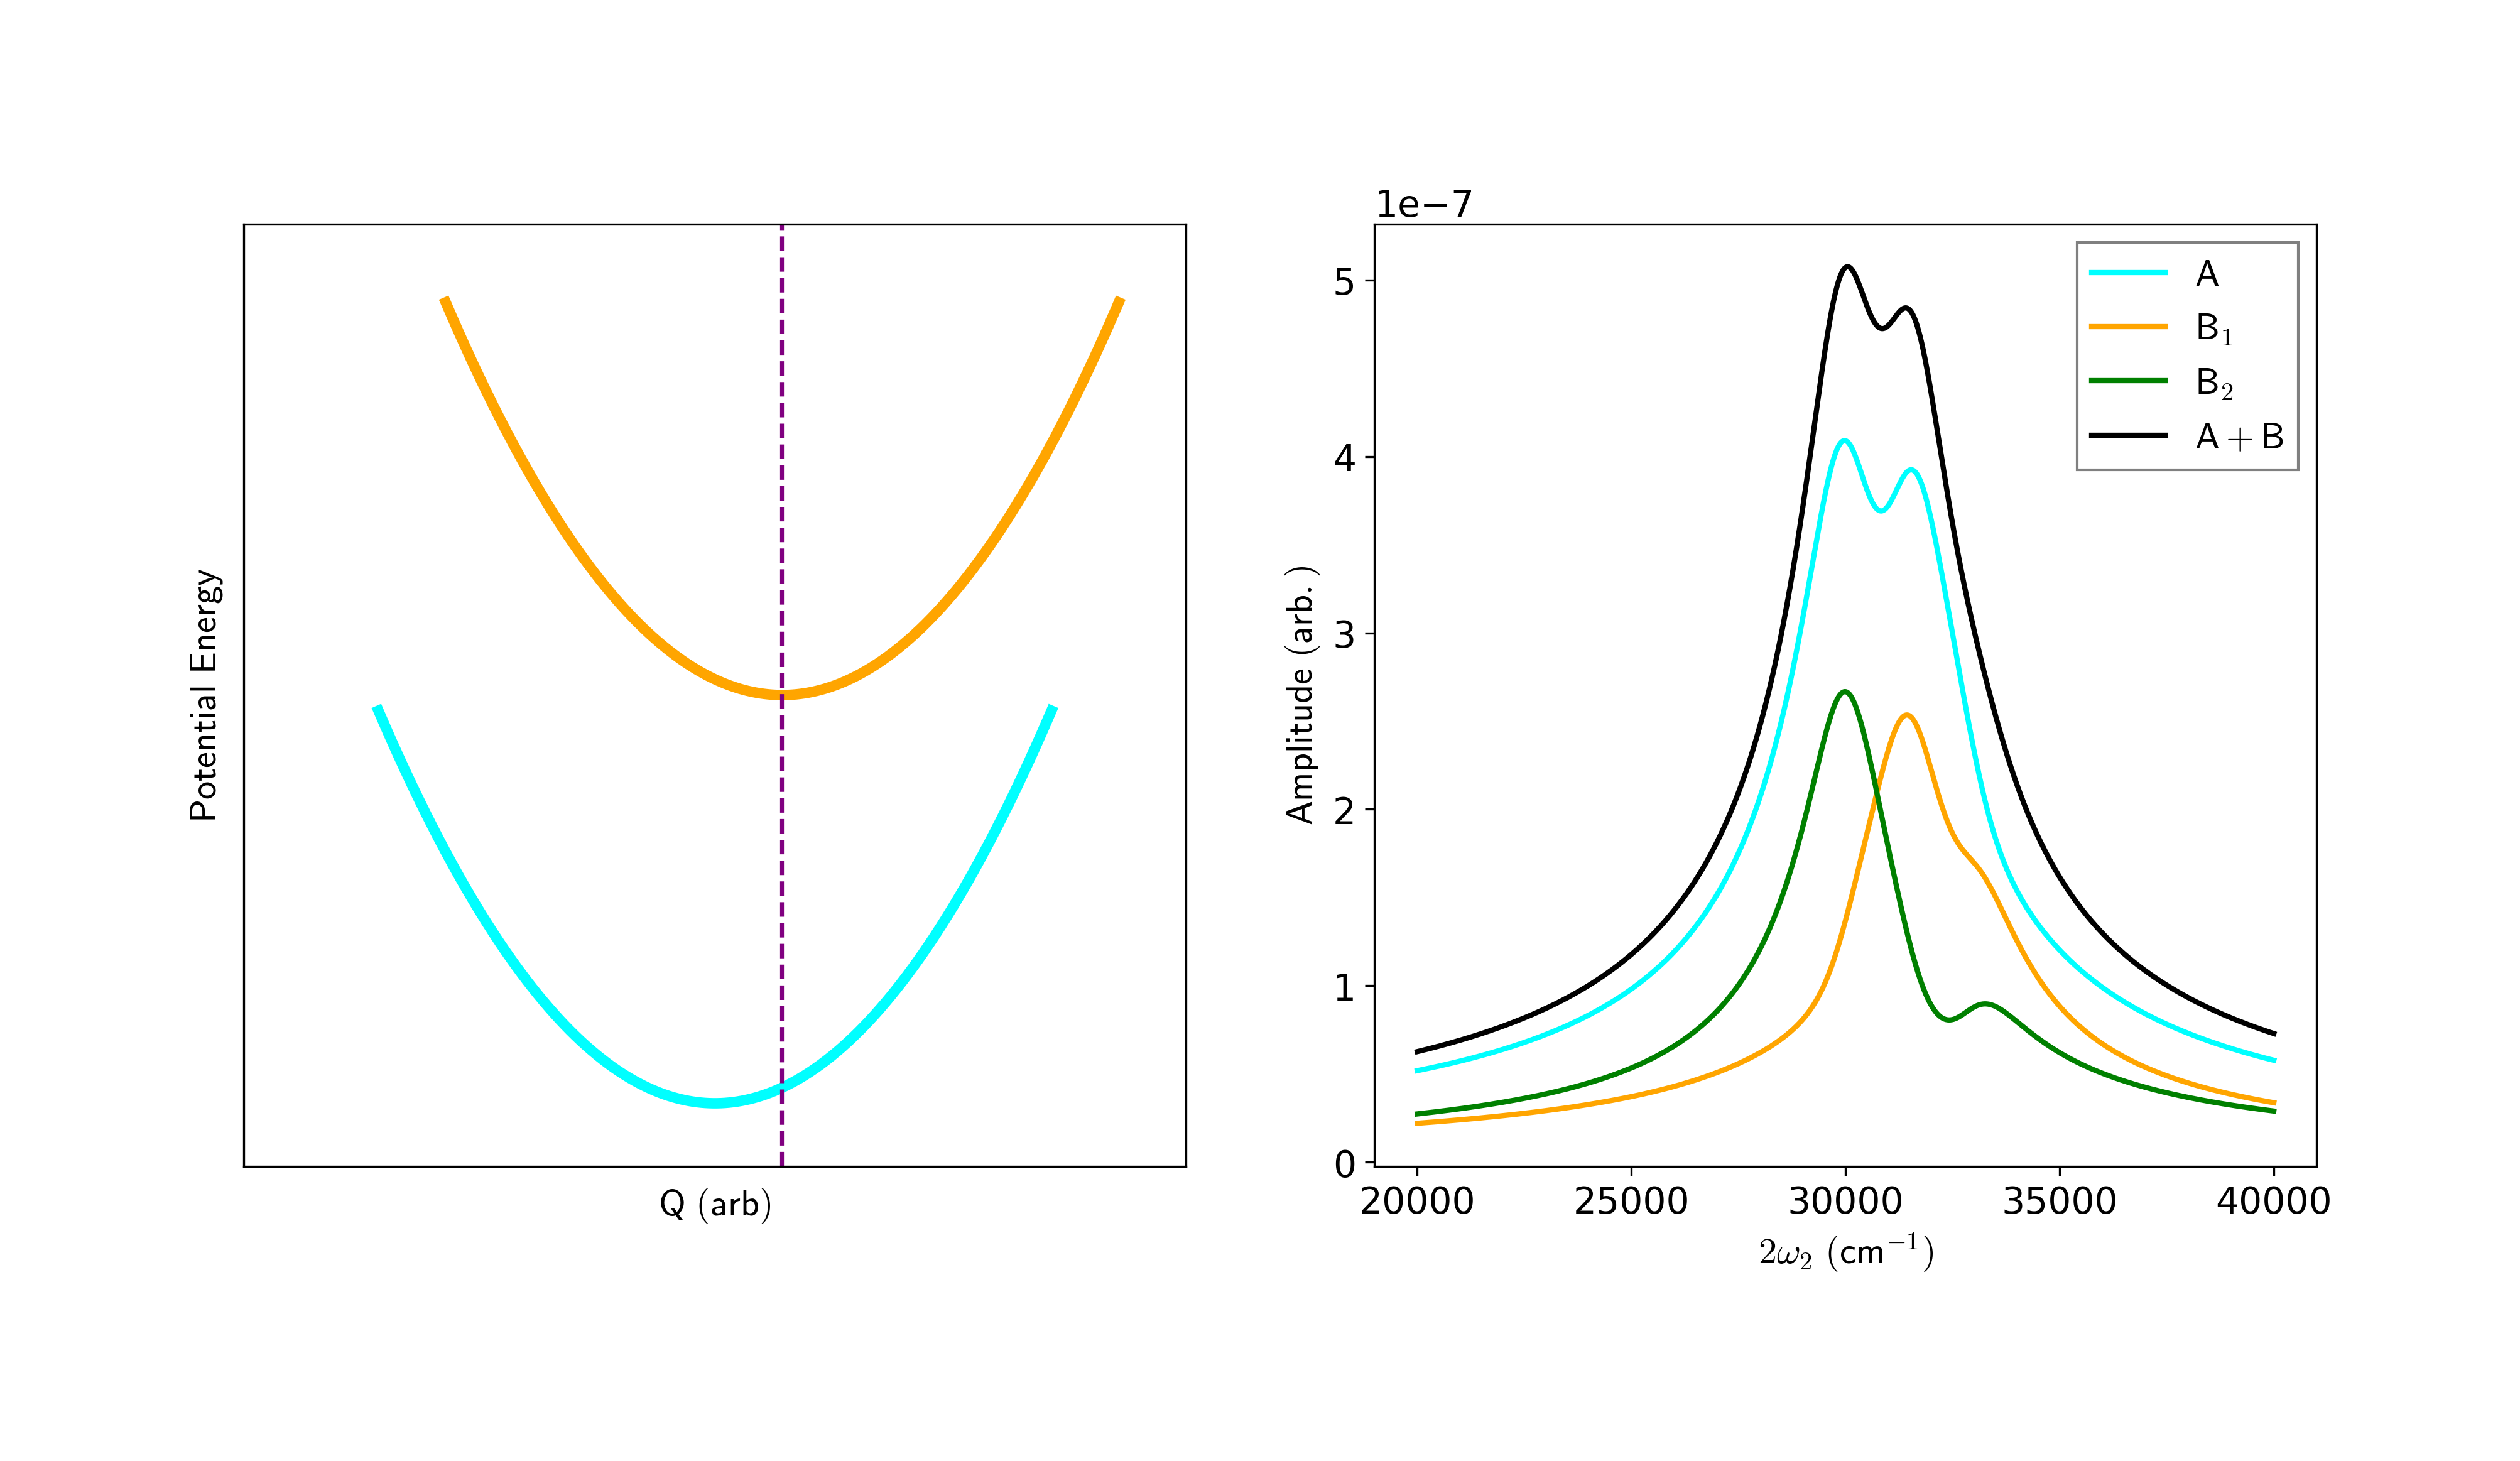
\includegraphics[width=6.66in]{drsive_spectrum.png}
	\caption{Contributions of $A, B$ (\autoref{ABterms_DR}) to HDFG spectrum for a simple two harmonic well system.
		(a) Potential energy surfaces for a two-well system, (b) 1D HDFG spectrum for $\Delta = 0.5$, $\omega_1 = \omega_{g1, g0}$, (c, d) real and imaginary parts of terms plotted in (b), respectively.
		The spectra are referenced to $\max{(A+B)}$. 
		It is assumed that $\omega_2 = \omega_3$, and that all molecular parameters used to simulate the spectra are positive.
		The vibrational states on the $|g)$ and $|e)$ manifolds are spaced 1600 cm$^{-1}$ apart, with the vibronic states $\ket{e,\tilde{v}'}$ given linewidths of 300 cm$^{-1}$ and $\omega_{eg}$ = 30000 cm$^{-1}$.
		Dotted lines in (b) denote the $\tilde{v}'$ = 0, 1, 2 vibronic resonances. 
		The vibronic one and two photon absorption operators are scaled such that $\max \left(\abs{B}/\abs{A}\right) \sim$ 0.1, following Chung and Ziegler. \cite{Ziegler1988}
		The Franck-Condon factor and Herzberg-Teller integral contributions to each of these terms are found in \autoref{T:contributions}.}
	\label{fig:doubres_spec}
\end{figure*}

\autoref{ABterms_DR} shows important selection rules for vibronic transitions in HDFG.
The $A$ term is allowed whenever an electronic transition has a one- and two- photon transition moment.
For centrosymmetric molecules, an electronic transition cannot be both one- and two- photon allowed by parity, so the $A$ term will vanish.
This makes HDFG a unique tool for studying the electronic structure of centrosymmetric species in isotropic media, as it is sensitive to non-Condon effects.\cite{Milojevich2011, Olson2018}
For an allowed electronic transition, the brightness of a vibronic resonance is controlled by overlap of ground and excited state vibrational wavefunctions (Franck-Condon factors).
The $A$ term relies on excited state perturbations to the vibrational wavefunctions; if the excited electronic state is minimally offset, $\langle 1 | \tilde{v}' \rangle \langle \tilde{v}' | 0 \rangle \rightarrow 0$ (\textit{vide infra}).
In the absence of an $A$ term, $B$ terms will dominate the HDFG response.

The signatures of vibronic coupling in the HDFG spectrum are made clear by using a simple model.
Using a two-well system described by $H = H_g |g) \left(g| + H_e |e\right) (e|$ where
\begin{subequations}\label{Hamiltonian}
	\begin{equation}
		H_g = \frac{\hbar \omega }{2} \left(p^2 + q^2 \right)
	\end{equation}
	and
	\begin{equation}
		H_e = \frac{\hbar \omega }{2} \left(p^2 +  (q-\Delta)^2 \right) + \hbar \omega_{eg}
	\end{equation}
\end{subequations}
for the ground ($H_g$) and first excited ($H_e$) states, where $p$ is the dimensionless momentum coordinate, $q = \sqrt{\frac{\omega}{\hbar}} Q$ is the dimensionless position coordinate, and $\Delta$ is the offset of the excited state surface relative to the ground state, the A and B contributions can be evaluated using Franck-Condon factors and Herzberg-Teller integrals (\autoref{fig:doubres_spec}a).
For simplicity, we restrict consideration to $v^\prime \in \{0,1,2\}$ and take $\Delta = 0.5$.

We assume the electronic state is both one and two photon allowed.
For this simulation, to enforce $\max \left(\abs{B}/\abs{A}\right) \sim$ 0.1 at $\Delta = 0.5$, we declare the coordinate dependencies
\begin{eqnarray}
	M^{ge}(q) = M^{ge}_0 \left(1 + 0.04 q + \order{q^2}\right),  \\
	\Lambda^{ge}(q) = \Lambda^{ge}_0 \left(1 + 0.04 q + \order{q^2}\right).
\end{eqnarray}
Here we expand $\vec{M}^{ij}$ about the equilibrium point of the ground state surface, $q = 0$.
Other reasonable expansion points choices include $q=\Delta$ and $q=\Delta/2$;\cite{Kundu2022}
so long as $\vec{M}^{ij}(q)$ and $\Lambda^{ge}(q)$ are roughly linear, the choice minimally affects the total calculation of $\gamma_{ijkl}$, but it does affect the weightings of $A$ and $B$ terms, primarily through changes in $\vec{M}_0^{ij}$ and the Herzberg-Teller integrals.
In summary, the expansion point somewhat affects the $A$ and $B$ spectra we show, but the overall spectrum $A+B$ is not affected by this choice.

\autoref{fig:doubres_spec}b shows the simulated HDFG spectrum for this two-well system where the hyper-Raman process is stimulated by two degenerate photons ($\omega_2 = \omega_3$). 
The spectrum selectively probes vibronic pathways from $\ket{g,0}$ to $\ket{g,1}$.
In the resonant region, the $A$ and $B$ terms contain character from all three possible transitions between $\ket{g,0}$, $\ket{e,\tilde{v}'}$ and $\ket{g,1}$. 
Significant contributions from $\ket{e,0}$ and $\ket{e,1}$ in the $A$ term spectrum correspond well with expectations given the relative wavefunction overlap in \autoref{fig:doubres_spec}a, tabulated in \autoref{T:contributions}. 
The overlaps are plotted as function of offset in Figure S2.
Similarly, the $B_1$ term is dominated by coupling with the $\ket{e,1}$ state and $B_2$ is dominated by coupling with the $\ket{e,0}$ state (\autoref{T:contributions}). 
Note that contributions involving $\ket{e,2}$ are suppressed relative to the $\ket{e,0}$ and $\ket{e,1}$ contributions in the $A$ and $B$ terms.
This is expected, considering the large change in quantum number when involving $\ket{e,2}$ and the offset of the potential wells in \autoref{Hamiltonian}.

In the pre-resonance region, both $A$ and $B$ terms die off as $\sim \Delta_{e\tilde{v}',gv}^{-1}$.
We point this out because a persistent belief in Raman analysis is that $A$ terms disappear and $B$ terms dominate when significantly detuned from electronic resonance.
The belief arises from the approximation that when $\abs{\omega_{e\tilde{v}',gv} - 2\omega_2} \gg 2\Gamma_{e\tilde{v}',gv}$, $A$ vanishes through a closure relationship.\cite{Neddersen1989}
As has been discussed elsewhere, however, this approximation is in many cases invalid, especially when vibrational energies are large, like those explored here.\cite{Warshel1977, Myers1982, Li1990, Gong2015}
This means that it could prove difficult to isolate $B$ terms when $A$ terms are present.

\begin{table*}[!htbp]
	\caption{\label{T:contributions} Franck-Condon and/or Herzberg-Teller contributions to $A$, $B_1$, $B_2$ terms between $\ket{g,0}$, $\ket{g,1}$ and vibronic states $\ket{e,\tilde{0}}$, $\ket{e,\tilde{1}}$, $\ket{e,\tilde{2}}$ for \autoref{Hamiltonian} with an offset $\Delta = 0.5$.
	The bra and ket labels are written according to their order in $A$, $B_1$, $B_2$ as written in \autoref{ABterms_DR}.
	The Franck-Condon factor and Herzberg-Teller integral products tabulated here are plotted in the Supporting Information (Figure S2) as a function of $\Delta$.}
	\begin{ruledtabular}
		\begin{tabular}{cccc}\label{fcht}
			$2\omega_2$ Electronic Resonance & $\ket{e,\tilde{0}}$ & $\ket{e,\tilde{1}}$ & $\ket{e,\tilde{2}}$\\
			\hline  
			$A$ 
			& $\langle 1 | \tilde{0} \rangle \langle \tilde{0} | 0 \rangle = 0.31 $  
			& $\langle 1 | \tilde{1} \rangle \langle \tilde{1} | 0 \rangle = -0.27 $ 
			& $\langle 1 | \tilde{2} \rangle \langle \tilde{2} | 0 \rangle = -0.04$\\
					
			$B_1$ 
			& $\langle 1 | \tilde{0} \rangle \mel{\tilde{0}}{Q}{0} = 0.08$ 
			& $\langle 1 | \tilde{1} \rangle \mel{\tilde{1}}{Q}{0} = 0.48$ 
			&$\langle 1 | \tilde{2} \rangle \mel{\tilde{2}}{Q}{0} = 0.14$\\
						
			$B_2$ 
			& $\mel{1}{Q}{\tilde{0}} \langle \tilde{0} | 0 \rangle = 0.70$  
			& $\mel{1}{Q}{\tilde{1}} \langle \tilde{1} | 0 \rangle = -0.07$ 
			& $\mel{1}{Q}{\tilde{2}} \langle \tilde{2} | 0 \rangle = 0.06$\\
		\end{tabular}
	\end{ruledtabular}
\end{table*}

The pre-resonance response is also dependent upon the specific molecular parameters that drive HDFG output.
The values of $\Delta$, $\omega_{g1, g0}$ and $\Gamma$ are system specific and affect the HDFG spectrum.
In the supporting information we demonstrate the impact of these parameters on the HDFG response using previously reported values (Figure S3). \cite{Myers1982, Brennan2024}
Based upon the response in Figure S3, $\Delta$, $\omega_{g1, g0}$ and $\Gamma$ have a significant impact on the resonant and pre-resonant HDFG response.
However, the driving terms in the HDFG response are the Franck-Condon factor and Herzberg-Teller integral products, which only depend upon $\Delta$.
Indeed, for some values of $\Delta$, most notably for $\Delta \rightarrow 0$, $A$ term products vanish, while $B$ term products are large (Figure S2).
As such, a small displacement of the electronic state from the ground state can allow for significant non-Condon behavior in pre-resonant HDFG response.

In the post-resonance region, the amplitude takes on an unusual lineshape.
This arises due to interference between the $A$ and $B$ terms; for our parameters, this interference is destructive in the post-resonance region (\autoref{fig:doubres_spec}c, d).
Examination of \autoref{ABterms_DR} shows that, while $A$ and $B$ terms share the same resonances, the relative phases of the contributions can vary due to the signs of $M^{ge}_0, \Lambda^{ge}_0, \frac{\partial M^{ge}}{\partial Q} , \frac{\partial \Lambda^{ge}}{\partial Q}$, as well as the Franck-Condon factor and Herzberg-Teller integral products, as discussed above. 
As a specific example, changing the sign of $M^{ge}_0$ eliminates the interference and restores the expected, purely Lorentzian lineshape (Figure S4).
Additionally, in this study, the reported spectra have considered only a single element of the HDFG $\gamma_{ijkl}$ tensor.
In bulk systems, the HDFG $\gamma_{ijkl}$ tensor must be averaged over molecular frame orientations (\autoref{eq:nfgamma}), which may also play a role in interference observed in an experimental HDFG spectrum.

\subsection{Inhomogeneity in HDFG}

An often unavoidable consequence in electronic spectroscopy is broadened line shapes due to a high density of vibronic modes and inhomogeneous broadening.
It is worthwhile to investigate the impact of inhomogeneity on HDFG response and the resultant lineshapes. 
In the discussion that follows, we assume that a ground state vibrational frequency, $\ket{g,v}$, experiences variations that are correlated to local changes in the environment and the frequencies of a vibronic $\ket{e,\tilde{v}'}$.
If the frequency of $\ket{g,v}$ is written as $\omega_{gv} + \xi$, where $\xi$ is some external strain (e.g. molecular collisions), then the frequency of $\ket{e,\tilde{v}'}$ is $\omega_{e\tilde{v}'} + c\xi$, where c is a shift coefficient.
We assume the fluctuations controlling the frequency variations are slow (the static limit), so that homogeneous lineshapes are unaffected by this fluctuation. 
When both states positively correlated, $c > 0$; similarly, modes are negatively correlated when $c < 0$.
For simplicity, we consider only c = $\pm$1.
To simplify discussion below, we map $\Delta^{3+2-1}_{e\tilde{v}', gv} \rightarrow \Delta^{3+2-1}_{ba}$ and $\Delta^{-1}_{g0,gv} \rightarrow \Delta^{-1}_{ga}$.
For clarity, we have reinstated the input pulse numbering to the $\Delta_{ij}$ terms for the discussion below (cf. \autoref{sivegamma}).

We investigate the impact of inhomogeneity on spectral output by convolving the HDFG output hyperpolarizability $\gamma_{ijkl}(\xi)$ with a normalized Lorentzian distribution $P(\xi)$ of half width $\sigma$ as \cite{Desiderio1979} 
\begin{widetext}
\begin{equation}\label{contour}
	\gamma_{ijkl} = \int_{-\infty}^\infty \mathrm{d}\xi \ P(\xi) \gamma_{ijkl}(\xi)
	= \frac{\sigma}{\pi}\int_{-\infty}^\infty \mathrm{d}\xi \frac{1}{\sigma^2 + \xi^2} \frac{\eta_{ijkl}}{\left(\Delta_{ga}^{-1} - \xi\right)\left(\Delta^{3+2-1}_{ba}+ c\xi\right)}
\end{equation} 
\end{widetext}
where $\eta_{ijkl}$ contains all values in \autoref{drgamma_notaylor} not dependent upon $\xi$.
While Gaussian distributions are commonly used as a phenomenological description of inhomogeneous broadening,\cite{RN307} Lorentzian distributions have successfully described inhomogeneous broadening in many multiply resonant coherent spectroscopies, and yield easily interpretable closed-form solutions. \cite{Dick83_1, Carlson1990line, RN410, Yurs2012}
\begin{widetext}
Evaluating \autoref{contour} for the HDFG pathway used above (\autoref{fig:sivewmel2}a) shows\footnote{See the supporting information for more details.} 
\begin{subequations}
	\begin{equation}\label{eq:linenarrowa}
		\gamma_{ijkl} = \frac{\eta_{ijkl}}{\left(\Delta_{ga}^{-1}-i\sigma \right) \left(\Delta^{3+2-1}_{ba}-i \sigma\right)}
	\end{equation}
for anti-correlated ($c = -1$) states, and
\begin{equation}\label{eq:linenarrowb}
	\gamma_{ijkl} = \frac{\eta_{ijkl}}{\Delta^{3+2-1}_{ba}+ i \sigma} \left(\frac{1}{\Delta_{ga}^{-1} - i \sigma} + \frac{2i\sigma}{(\Delta^{3+2-1}_{ba} - i \sigma)(\Delta_{ga}^{-1} + \Delta^{3+2-1}_{ba})}\right)
\end{equation}
for correlated ($c = 1$) states. 
\end{subequations}
\end{widetext}
For anti-correlated modes (\autoref{eq:linenarrowa}), we see the inhomogeneous envelope width $\sigma$ is added to the linewidth of each resonance (e.g., $\Gamma_{ga} \rightarrow \Gamma_{ga} + \sigma$).
In other words, HDFG spectra of anti-correlated vibrational and vibronic modes will contain the same inhomogeneity present in a typical 1D spectrum.

The output for correlated modes shows the presence of a new term, $\frac{2i\sigma}{\Delta_{ga} + \Delta_{ba}}$, along with other terms where the inhomogeneous width is added to the resonance linewidth. 
However, unlike the other terms, the $\frac{2i\sigma}{\Delta_{ga} + \Delta_{ba}}$ term is amplified by the width of the inhomogeneous envelope ($\sigma$) and has a linewidth $\Gamma_{ba} + \Gamma_{ga}$.
As a result, this term will dominate over the other terms. 
Since the linewidth of the dominant term, $\Gamma_{ba} + \Gamma_{ga}$, is a direct report on the linewidth of the coupled modes, this is evidence of line-narrowing in the HDFG spectrum. \cite{RN103}
Or, the HDFG pathway considered in this work line-narrows correlated modes. 
For all cases, it is useful to note that in the limit of zero inhomogeneity ($\sigma \rightarrow 0$), the results in \autoref{drgamma_notaylor} are restored.
These results are consistent with the idea that non-parametric, non-linear spectroscopies line-narrow correlated modes. \cite{Dick83_1, Carlson1990line}

Although \autoref{eq:linenarrowb} identifies that non-parametric HDFG line-narrows correlated modes, these results are only valid in limits where the input pulses weakly populate excited states.
When resonant pulses are significantly longer than the dephasing time of some state, then that state can become significantly populated.
Excited state population effects are particularly important for understanding the spectroscopy of electronic states using input pulses with pulse widths significantly longer than dephasing times. \cite{RN471}
Excited state populations can feed other modes, including the ground state and other vibrational/vibronic modes, inducing higher order processes.\cite{RN471}
These feeding mechanisms can induce line-narrowing properties in spectroscopies that cannot line-narrow in third order perturbation theory.\cite{RN471, RN410}

\section{Quantitative Aspects of HDFG}\label{quant}

\subsection{vSFG detection levels are adequate for HDFG}
Can vSFG experimental setups detect HDFG signals?
SFG experiments typically leverage the surface selectivity of $\chi^{(2)}$ polarizations, which results in extremely small emission volumes, so SFG setups are typically quite sensitive.
However, HDFG is a weak $\chi^{(3)}$ process because it depends upon hyper-Raman cross-sections, which are commonly several orders of magnitude weaker than corresponding Raman transitions.\cite{RN515}
Since HDFG can be performed as a two-beam experiment, it is useful to identify whether vSFG and HDFG responses are similar to quantify hyper-Raman-based FWM response from bulk, isotropic systems.
To evaluate the feasibility of HDFG for vSFG practitioners, we have compared the relative output of each process using nominal parameters. 
As calculated in \autoref{appendixA}, HDFG's weak $\chi^{(3)}$ value and SFG's low emission cancel somewhat, so that the output polarization of HDFG and vSFG are comparable ($\abs{P_\text{vSFG} / P_\text{HDFG}} \sim 1$).
Transient HDFG, or IR-pump-HDFG-probe, analogous to IR-pump-vSFG-probe, is therefore also feasible under similar experimental conditions, and provides vSFG practitioners a simple method to measure bulk dynamics without significant changes in an experimental setup. 
Therefore, HDFG is a feasible spectroscopy for practitioners of vSFG both in terms of experimental setup and detection feasibility.


\subsection{Extraction of hyper-Raman hyperpolarizability}

Compared to $\vec{\mu}$ and $\alpha_{ij}$, it is difficult to measure $\beta_{ijk}$ values through spontaneous hyper-Raman experiments.\cite{Kelley2010}
Only a few experimental determinations of $\beta_{ijk}$ for vibrational modes have been performed.\cite{Xu1997, Shoute2005, Kelley2010}
Methods reported in the literature to measure absolute hyper-Raman polarizabilities depend upon external standards, such as hyperpolarizabilities or two-photon excited fluorescence of known samples, also difficult to measure. \cite{Kelley2010} 
In the method introduced by Levenson and Bloembergen (Bloembergen interferometry experiment), an internal standard interferes with the resonant lineshape of a $\chi^{(3)}$ process. \cite{Levenson1974_1, Levenson1974_2}
Self-heterodyning of the internal standard signal measures $\chi^{(3)}$ and does not require measurement of absolute intensities. 
Since the Bloembergen interferometry experiment only relies on the third order susceptibility for measured species (e.g., benzene or CaF$_2$),\cite{Levenson1974_2} it is possible to use quantitative four wave mixing spectroscopy to calculate $\beta_{ijk}$ values for infrared active vibrations.
It is thus useful to investigate how a treatment of orientational averaging can extract $\beta_{ijk}$ from the HDFG $\chi^{(3)}_{IJKL}$ expression.

Using \autoref{eq:nfgamma} and \autoref{sivebeta}, we can write
\begin{equation}\label{chi3}
		\chi^{(3)}_{IJKL} = -\frac{NF}{4D \hbar \varepsilon_0 \Delta_{gv}} \langle \beta_{ijk} \mu_l \rangle_{IJKL} \rho^{(0)}_{gg}\\
\end{equation}
For simplicity, we take $\rho^{(0)}_{gg} = 1$.
Orientational averaging shows polarization schemes can isolate specific linear combinations of different $\beta_{ijk}$ terms. \cite{Bersohn1966, Kauranen1996}
Substituting in \autoref{SIVEselection}, we see
\begin{equation}\label{betasive}
	\left\langle \frac{\partial \beta_{ijk}}{\partial Q_v} {\frac{\partial \mu_l}{\partial Q_v}} \right\rangle_{IJKL} = -\frac{8D \varepsilon_0}{NF}  {\Gamma_{gv} \omega_{vg}} \chi^{(3)}_{IJKL}
\end{equation}
Since $\abs{\partial \mu_l / \partial Q}$ values can be extracted from FT-IR spectra and $\chi^{(3)}$ can be extracted through the Bloembergen interferometry experiment,\cite{Levenson1974_1, Levenson1974_2, RN459} HDFG can give quantitative information on the magnitude of $\frac{\partial \beta_{ijk}}{\partial Q}$ for infrared active vibrations.
Additionally, by using non-degenerate input frequencies to stimulate the hyper-Raman transition, the asymmetric properties of $\beta_{ijk}$ can be examined and quantified. \cite{Denisov1986, Kozich2007}
These quantitative aspects of HDFG could prove useful for examining how well computational methods calculate $\beta_{ijk}$ values.

\section{Conclusions}\label{conclusion}
Coherent vibrational, hyper-Raman coherent four wave mixing spectroscopies are identified and discussed.
Hyper difference frequency generation (HDFG) possesses infrared absorption and vibronic hyper-Raman scattering selection rules.
As a result, HDFG output is sensitive to the relative overlap of potential energy surfaces.
If the potential energy surface is not significantly modulated along the vibrational coordinate of interest, then output is dominated by $A$ term resonances, or Franck-Condon contributions.
However, $B$ term resonances, or Herzberg-Teller contributions, dominate in centrosymmetric media, as $A$ term resonances vanish in centrosymmetric media through parity constraints.
A treatment of inhomogeneous broadening shows that for positively correlated vibrational and vibronic resonances, HDFG line narrows the spectral output, eliminating inhomogeneous broadening. 
As a result, HDFG possesses site-selective properties analogous to those of coherent Raman spectroscopies, which can allow for a thorough analysis of vibronic coupling schemes in isotropic systems.
We show that HDFG provides alternative methods to extract the hyper-Raman hyperpolarizability of infrared active vibrations. 
Since HDFG is approachable as a two-beam experiment, analogous to vibrational sum-frequency generation, and phase-matchable in media with normal dispersion, HDFG should be applicable towards understanding vibrational spectroscopy and dynamics, e.g. single quantum coherence free induction decay dynamics, in a variety of relevant molecular and materials systems.  

\section{Data Availability Statement}
The workup scripts that support this study are permissively licensed and available for reuse at \href{https://osf.io/2amkq/}{https://osf.io/2amkq/}.

\section{Acknowledgments}
This work received support from the National Science Foundation (Grant no. CHE-2203290).
R.P.M. acknowledges support from the National Science Foundation Graduate Research Fellowship Program (Grant no. DGE-2137424). 

\section{Supplemental Information}
See the supporting information for details on deriving closed-form solutions to Herzberg-Teller integrals, HDFG spectrum dependence on $\Delta$, and evaluation of \autoref{contour}.

\section{Appendix: Comparison of vSFG and two-beam HDFG output}\label{appendixA}
To motivate the application of HDFG spectroscopy, we perform a calculation to compare vibrationally resonant two-color HDFG and vSFG output, where absorption effects are neglected for simplicity.
vSFG is a $\chi^{(2)}$ technique, when only vibrationally resonant, whose output scales as $\chi^{(2)}_{IJK} \sim \langle \alpha_{ij} \mu_k \rangle$, where $\alpha_{ij}$ is the Raman polarizability tensor.
The output polarizations for two-beam vSFG and HDFG, respectively, under the electric dipole approximation, and assuming exponential dephasing, when vibrationally resonant are written as:
	 	\begin{subequations}
		 	\begin{equation}\label{PSFG}
		 		\begin{split}
		 		\abs{P^{(2)}_{\text{vSFG}}} &= \frac{N_\text{surf}}{\ell} \abs{ \frac{F_{\text{vSFG}} \langle \alpha_{ij}\mu_{k} \rangle }{2D' \varepsilon_0 \hbar i \Gamma} E(\omega_2)E(\omega_1) } 
		 		\end{split}
			 \end{equation}
		 	\begin{equation}
		 		\begin{split}
			 		\abs{P^{(3)}_{\text{HDFG}}} &= 6 N_\text{bulk} \abs{{ \frac{-F_{\text{HDFG}} \langle \beta_{ijk} \mu_{l} \rangle }{4D \varepsilon_0 \hbar i \Gamma} E{(\omega_2)}E(\omega_2)E(-\omega_1) }}, 
		 		\end{split}
			 \end{equation}
		 \end{subequations}
where N$_\text{bulk}$ is the bulk number density ($\sim$ 10$^{28}$ m$^{-3}$ for liquid H$_2$O at room temperature), N$_\text{surf}$ is the surface number density ($\sim$ 10$^{16}$ m$^{-2}$ for H$_2$O adsorbed at quartz at room temperature),\cite{Du1994} $D'$ is the SFG degeneracy factor, and $\Gamma$ is the vibrational dephasing rate.
For a two-beam experiment, $D' = 2$ and $D = 3$.
The HDFG output gains a multiplicative factor of 6 because six singly resonant HDFG processes contribute at pulse overlap.
	
For simplicity, we assume that $\chi^{(2)}$ is a spatial constant. 
We take the film thickness ($\ell$) probed by vSFG to be 1 nm, much less than the vSFG coherence length.\cite{RN133}
A normal dispersion curve is assumed so that $n(\omega_1+\omega_2) \approx n(2\omega_2-\omega_1)$.
To simplify analysis, orientational averaging is ignored (e.g., $\langle \beta_{ijk} \mu_{l} \rangle \approx \beta \mu$) and the input and output fields are taken to be co-polarized, so that
\begin{equation}
	P_\text{ratio} \equiv \frac{\abs{P^{(3)}_{\text{HDFG}}}}{\abs{P^{(2)}_{\text{vSFG}}}} \approx 2 \frac{N_\text{bulk}}{N_\text{surf}} \ell \abs{\frac{\left(n(\omega_2)\right)^2 + 1}{3}} \frac{\beta}{\alpha} E(\omega_2) \sim 10^3 \frac{\beta}{\alpha} E(\omega_2)\\
\end{equation}
Ziegler has noted that for a field with intensity 10 GW/cm$^{2}$, $\frac{\beta E}{\alpha} \sim 10^{-3} $ for vibrational modes when detuned from electronic resonances, i.e., singly resonant response. \cite{RN515}
Such an intensity is easily obtained using modern ultrafast sources.
Under these conditions, $P_\text{ratio} \sim 1$, or the HDFG output is similar to that of vSFG, assuming only interfacial contributions in vSFG.
It is important to note that this calculation assumed negligible dipole and Raman polarizability dependence upon the distance from surface normal, ignored orientational averaging effects, and presumed equivalence of local field factors, all of which can significantly reduce output from either process. 
Nevertheless, since HDFG produces a similar number of photons as vSFG, HDFG is a viable technique for investigating bulk systems.
Laboratories which use vSFG to investigate interfacial species at buried interfaces thus have the ingredients necessary to perform a HDFG experiment in a transmission geometry. \cite{Piontek2023_1}
This method provides vSFG practitioners the ability to measure spectra and dephasing dynamics in isotropic media without many meaningful changes in their optical setup, and thus compare spectroscopy and dephasing in the bulk and at the interface.



\section{References}
% Create the reference section using BibTeX:
%\bibliography{library.bib}
%apsrev4-2.bst 2019-01-14 (MD) hand-edited version of apsrev4-1.bst
%Control: key (0)
%Control: author (72) initials jnrlst
%Control: editor formatted (1) identically to author
%Control: production of article title (-1) disabled
%Control: page (0) single
%Control: year (1) truncated
%Control: production of eprint (0) enabled
\begin{thebibliography}{112}%
	\makeatletter
	\providecommand \@ifxundefined [1]{%
		\@ifx{#1\undefined}
	}%
	\providecommand \@ifnum [1]{%
		\ifnum #1\expandafter \@firstoftwo
		\else \expandafter \@secondoftwo
		\fi
	}%
	\providecommand \@ifx [1]{%
		\ifx #1\expandafter \@firstoftwo
		\else \expandafter \@secondoftwo
		\fi
	}%
	\providecommand \natexlab [1]{#1}%
	\providecommand \enquote  [1]{``#1''}%
	\providecommand \bibnamefont  [1]{#1}%
	\providecommand \bibfnamefont [1]{#1}%
	\providecommand \citenamefont [1]{#1}%
	\providecommand \href@noop [0]{\@secondoftwo}%
	\providecommand \href [0]{\begingroup \@sanitize@url \@href}%
	\providecommand \@href[1]{\@@startlink{#1}\@@href}%
	\providecommand \@@href[1]{\endgroup#1\@@endlink}%
	\providecommand \@sanitize@url [0]{\catcode `\\12\catcode `\$12\catcode
		`\&12\catcode `\#12\catcode `\^12\catcode `\_12\catcode `\%12\relax}%
	\providecommand \@@startlink[1]{}%
	\providecommand \@@endlink[0]{}%
	\providecommand \url  [0]{\begingroup\@sanitize@url \@url }%
	\providecommand \@url [1]{\endgroup\@href {#1}{\urlprefix }}%
	\providecommand \urlprefix  [0]{URL }%
	\providecommand \Eprint [0]{\href }%
	\providecommand \doibase [0]{https://doi.org/}%
	\providecommand \selectlanguage [0]{\@gobble}%
	\providecommand \bibinfo  [0]{\@secondoftwo}%
	\providecommand \bibfield  [0]{\@secondoftwo}%
	\providecommand \translation [1]{[#1]}%
	\providecommand \BibitemOpen [0]{}%
	\providecommand \bibitemStop [0]{}%
	\providecommand \bibitemNoStop [0]{.\EOS\space}%
	\providecommand \EOS [0]{\spacefactor3000\relax}%
	\providecommand \BibitemShut  [1]{\csname bibitem#1\endcsname}%
	\let\auto@bib@innerbib\@empty
	%</preamble>
	\bibitem [{\citenamefont {Cho}(2008)}]{Cho2008}%
	\BibitemOpen
	\bibfield  {author} {\bibinfo {author} {\bibfnamefont {M.}~\bibnamefont
			{Cho}},\ }\href {https://doi.org/10.1021/cr078377b} {\bibfield  {journal}
		{\bibinfo  {journal} {Chemical Reviews}\ }\textbf {\bibinfo {volume} {108}},\
		\bibinfo {pages} {1331} (\bibinfo {year} {2008})}\BibitemShut {NoStop}%
	\bibitem [{\citenamefont {Oudar}\ and\ \citenamefont {Shen}(1980)}]{RN307}%
	\BibitemOpen
	\bibfield  {author} {\bibinfo {author} {\bibfnamefont {J.~L.}\ \bibnamefont
			{Oudar}}\ and\ \bibinfo {author} {\bibfnamefont {Y.~R.}\ \bibnamefont
			{Shen}},\ }\href {https://doi.org/10.1103/PhysRevA.22.1141} {\bibfield
		{journal} {\bibinfo  {journal} {Phys. Rev. A}\ }\textbf {\bibinfo {volume}
			{22}},\ \bibinfo {pages} {1141} (\bibinfo {year} {1980})}\BibitemShut
	{NoStop}%
	\bibitem [{\citenamefont {Nguyen}\ and\ \citenamefont {Wright}(1985)}]{RN281}%
	\BibitemOpen
	\bibfield  {author} {\bibinfo {author} {\bibfnamefont {D.~C.}\ \bibnamefont
			{Nguyen}}\ and\ \bibinfo {author} {\bibfnamefont {J.~C.}\ \bibnamefont
			{Wright}},\ }\href
	{https://doi.org/https://doi.org/10.1016/0009-2614(85)80208-6} {\bibfield
		{journal} {\bibinfo  {journal} {Chemical Physics Letters}\ }\textbf {\bibinfo
			{volume} {117}},\ \bibinfo {pages} {224} (\bibinfo {year}
		{1985})}\BibitemShut {NoStop}%
	\bibitem [{\citenamefont {Wright}\ \emph {et~al.}(1991)\citenamefont {Wright},
		\citenamefont {Carlson}, \citenamefont {Hurst}, \citenamefont {Steehler},
		\citenamefont {Riebe}, \citenamefont {Price}, \citenamefont {Nguyen},\ and\
		\citenamefont {Lee}}]{RN103}%
	\BibitemOpen
	\bibfield  {author} {\bibinfo {author} {\bibfnamefont {J.~C.}\ \bibnamefont
			{Wright}}, \bibinfo {author} {\bibfnamefont {R.~J.}\ \bibnamefont {Carlson}},
		\bibinfo {author} {\bibfnamefont {G.~B.}\ \bibnamefont {Hurst}}, \bibinfo
		{author} {\bibfnamefont {J.~K.}\ \bibnamefont {Steehler}}, \bibinfo {author}
		{\bibfnamefont {M.~T.}\ \bibnamefont {Riebe}}, \bibinfo {author}
		{\bibfnamefont {B.~B.}\ \bibnamefont {Price}}, \bibinfo {author}
		{\bibfnamefont {D.~C.}\ \bibnamefont {Nguyen}},\ and\ \bibinfo {author}
		{\bibfnamefont {S.~H.}\ \bibnamefont {Lee}},\ }\href
	{https://doi.org/10.1080/01442359109353262} {\bibfield  {journal} {\bibinfo
			{journal} {International Reviews in Physical Chemistry}\ }\textbf {\bibinfo
			{volume} {10}},\ \bibinfo {pages} {349} (\bibinfo {year} {1991})}\BibitemShut
	{NoStop}%
	\bibitem [{\citenamefont {Gaynor}\ and\ \citenamefont
		{Khalil}(2017)}]{Gaynor2017}%
	\BibitemOpen
	\bibfield  {author} {\bibinfo {author} {\bibfnamefont {J.~D.}\ \bibnamefont
			{Gaynor}}\ and\ \bibinfo {author} {\bibfnamefont {M.}~\bibnamefont
			{Khalil}},\ }\href {https://doi.org/10.1063/1.4991745} {\bibfield  {journal}
		{\bibinfo  {journal} {Journal of Chemical Physics}\ }\textbf {\bibinfo
			{volume} {147}},\ \bibinfo {pages} {094202} (\bibinfo {year}
		{2017})}\BibitemShut {NoStop}%
	\bibitem [{\citenamefont {Mandal}\ \emph {et~al.}(2018)\citenamefont {Mandal},
		\citenamefont {Ng~Pack}, \citenamefont {Shah}, \citenamefont {Erramilli},\
		and\ \citenamefont {Ziegler}}]{Ziegler2018}%
	\BibitemOpen
	\bibfield  {author} {\bibinfo {author} {\bibfnamefont {A.}~\bibnamefont
			{Mandal}}, \bibinfo {author} {\bibfnamefont {G.}~\bibnamefont {Ng~Pack}},
		\bibinfo {author} {\bibfnamefont {P.~P.}\ \bibnamefont {Shah}}, \bibinfo
		{author} {\bibfnamefont {S.}~\bibnamefont {Erramilli}},\ and\ \bibinfo
		{author} {\bibfnamefont {L.~D.}\ \bibnamefont {Ziegler}},\ }\href
	{https://doi.org/10.1103/PhysRevLett.120.103401} {\bibfield  {journal}
		{\bibinfo  {journal} {Phys. Rev. Lett.}\ }\textbf {\bibinfo {volume} {120}},\
		\bibinfo {pages} {103401} (\bibinfo {year} {2018})}\BibitemShut {NoStop}%
	\bibitem [{\citenamefont {Song}\ \emph {et~al.}(2019)\citenamefont {Song},
		\citenamefont {Schubert}, \citenamefont {Maret}, \citenamefont {Burdick},
		\citenamefont {Dunietz}, \citenamefont {Geva},\ and\ \citenamefont
		{Ogilvie}}]{Ogilvie2019}%
	\BibitemOpen
	\bibfield  {author} {\bibinfo {author} {\bibfnamefont {Y.}~\bibnamefont
			{Song}}, \bibinfo {author} {\bibfnamefont {A.}~\bibnamefont {Schubert}},
		\bibinfo {author} {\bibfnamefont {E.}~\bibnamefont {Maret}}, \bibinfo
		{author} {\bibfnamefont {R.~K.}\ \bibnamefont {Burdick}}, \bibinfo {author}
		{\bibfnamefont {B.~D.}\ \bibnamefont {Dunietz}}, \bibinfo {author}
		{\bibfnamefont {E.}~\bibnamefont {Geva}},\ and\ \bibinfo {author}
		{\bibfnamefont {J.~P.}\ \bibnamefont {Ogilvie}},\ }\href
	{https://doi.org/10.1039/C9SC02329A} {\bibfield  {journal} {\bibinfo
			{journal} {Chem. Sci.}\ }\textbf {\bibinfo {volume} {10}},\ \bibinfo {pages}
		{8143} (\bibinfo {year} {2019})}\BibitemShut {NoStop}%
	\bibitem [{\citenamefont {Vietze}\ \emph {et~al.}(2021)\citenamefont {Vietze},
		\citenamefont {Backus}, \citenamefont {Bonn},\ and\ \citenamefont
		{Grechko}}]{Bonn2021}%
	\BibitemOpen
	\bibfield  {author} {\bibinfo {author} {\bibfnamefont {L.}~\bibnamefont
			{Vietze}}, \bibinfo {author} {\bibfnamefont {E.~H.~G.}\ \bibnamefont
			{Backus}}, \bibinfo {author} {\bibfnamefont {M.}~\bibnamefont {Bonn}},\ and\
		\bibinfo {author} {\bibfnamefont {M.}~\bibnamefont {Grechko}},\ }\href
	{https://doi.org/10.1063/5.0047918} {\bibfield  {journal} {\bibinfo
			{journal} {Journal of Chemical Physics}\ }\textbf {\bibinfo {volume} {154}},\
		\bibinfo {pages} {174201} (\bibinfo {year} {2021})}\BibitemShut {NoStop}%
	\bibitem [{\citenamefont {Daniels}\ \emph {et~al.}(2022)\citenamefont
		{Daniels}, \citenamefont {Wells},\ and\ \citenamefont {Chen}}]{RN325}%
	\BibitemOpen
	\bibfield  {author} {\bibinfo {author} {\bibfnamefont {D.~A.}\ \bibnamefont
			{Daniels}}, \bibinfo {author} {\bibfnamefont {T.~A.}\ \bibnamefont {Wells}},\
		and\ \bibinfo {author} {\bibfnamefont {P.~C.}\ \bibnamefont {Chen}},\ }\href
	{https://doi.org/10.1063/5.0109084} {\bibfield  {journal} {\bibinfo
			{journal} {Journal of Chemical Physics}\ }\textbf {\bibinfo {volume} {157}},\
		\bibinfo {pages} {184201} (\bibinfo {year} {2022})}\BibitemShut {NoStop}%
	\bibitem [{\citenamefont {Chen}\ and\ \citenamefont
		{Daniels}(2024)}]{Chen2024}%
	\BibitemOpen
	\bibfield  {author} {\bibinfo {author} {\bibfnamefont {P.~C.}\ \bibnamefont
			{Chen}}\ and\ \bibinfo {author} {\bibfnamefont {D.~A.}\ \bibnamefont
			{Daniels}},\ }\href {https://doi.org/10.1021/acs.jpclett.3c03254} {\bibfield
		{journal} {\bibinfo  {journal} {Journal of Physical Chemistry Letters}\
		}\textbf {\bibinfo {volume} {15}},\ \bibinfo {pages} {1234} (\bibinfo {year}
		{2024})}\BibitemShut {NoStop}%
	\bibitem [{\citenamefont {Dhar}\ \emph {et~al.}(1994)\citenamefont {Dhar},
		\citenamefont {Rogers},\ and\ \citenamefont {Nelson}}]{Dhar1994}%
	\BibitemOpen
	\bibfield  {author} {\bibinfo {author} {\bibfnamefont {L.}~\bibnamefont
			{Dhar}}, \bibinfo {author} {\bibfnamefont {J.~A.}\ \bibnamefont {Rogers}},\
		and\ \bibinfo {author} {\bibfnamefont {K.~A.}\ \bibnamefont {Nelson}},\
	}\href {https://doi.org/10.1021/cr00025a006} {\bibfield  {journal} {\bibinfo
			{journal} {Chemical Reviews}\ }\textbf {\bibinfo {volume} {94}},\ \bibinfo
		{pages} {157} (\bibinfo {year} {1994})}\BibitemShut {NoStop}%
	\bibitem [{\citenamefont {Zhao}\ and\ \citenamefont {Wright}(1999)}]{RN345}%
	\BibitemOpen
	\bibfield  {author} {\bibinfo {author} {\bibfnamefont {W.}~\bibnamefont
			{Zhao}}\ and\ \bibinfo {author} {\bibfnamefont {J.~C.}\ \bibnamefont
			{Wright}},\ }\href {https://doi.org/10.1103/PhysRevLett.83.1950} {\bibfield
		{journal} {\bibinfo  {journal} {Phys. Rev. Lett.}\ }\textbf {\bibinfo
			{volume} {83}},\ \bibinfo {pages} {1950} (\bibinfo {year}
		{1999})}\BibitemShut {NoStop}%
	\bibitem [{\citenamefont {Cho}(2000)}]{Cho2000}%
	\BibitemOpen
	\bibfield  {author} {\bibinfo {author} {\bibfnamefont {M.}~\bibnamefont
			{Cho}},\ }\href {https://doi.org/10.1103/PhysRevA.61.023406} {\bibfield
		{journal} {\bibinfo  {journal} {Phys. Rev. A}\ }\textbf {\bibinfo {volume}
			{61}},\ \bibinfo {pages} {023406} (\bibinfo {year} {2000})}\BibitemShut
	{NoStop}%
	\bibitem [{\citenamefont {Boyle}\ \emph {et~al.}(2014)\citenamefont {Boyle},
		\citenamefont {Neff-Mallon}, \citenamefont {Handali},\ and\ \citenamefont
		{Wright}}]{RN491}%
	\BibitemOpen
	\bibfield  {author} {\bibinfo {author} {\bibfnamefont {E.~S.}\ \bibnamefont
			{Boyle}}, \bibinfo {author} {\bibfnamefont {N.~A.}\ \bibnamefont
			{Neff-Mallon}}, \bibinfo {author} {\bibfnamefont {J.~D.}\ \bibnamefont
			{Handali}},\ and\ \bibinfo {author} {\bibfnamefont {J.~C.}\ \bibnamefont
			{Wright}},\ }\href {https://doi.org/10.1021/jp5018554} {\bibfield  {journal}
		{\bibinfo  {journal} {Journal of Physical Chemistry A}\ }\textbf {\bibinfo
			{volume} {118}},\ \bibinfo {pages} {3112} (\bibinfo {year}
		{2014})}\BibitemShut {NoStop}%
	\bibitem [{\citenamefont {Lee}\ and\ \citenamefont {Albrecht}(1985)}]{RN286}%
	\BibitemOpen
	\bibfield  {author} {\bibinfo {author} {\bibfnamefont {D.}~\bibnamefont
			{Lee}}\ and\ \bibinfo {author} {\bibfnamefont {A.~C.}\ \bibnamefont
			{Albrecht}},\ }\bibinfo {title} {A {U}nified {V}iew of {R}aman, {R}esonance
		{R}aman, and {F}luorescence {S}pectroscopy (and their {A}nalogues in
		{T}wo-{P}hoton {A}bsorption)},\ in\ \href@noop {} {\emph {\bibinfo
			{booktitle} {Advances in Infrared and Raman Spectroscopies}}},\ \bibinfo
	{editor} {edited by\ \bibinfo {editor} {\bibfnamefont {R.}~\bibnamefont
			{Clark}}\ and\ \bibinfo {editor} {\bibfnamefont {R.}~\bibnamefont {Hester}}}\
	(\bibinfo  {publisher} {Wiley},\ \bibinfo {address} {New York},\ \bibinfo
	{year} {1985})\ pp.\ \bibinfo {pages} {179--213}\BibitemShut {NoStop}%
	\bibitem [{\citenamefont {Terhune}\ \emph {et~al.}(1965)\citenamefont
		{Terhune}, \citenamefont {Maker},\ and\ \citenamefont
		{Savage}}]{Terhune1965}%
	\BibitemOpen
	\bibfield  {author} {\bibinfo {author} {\bibfnamefont {R.~W.}\ \bibnamefont
			{Terhune}}, \bibinfo {author} {\bibfnamefont {P.~D.}\ \bibnamefont {Maker}},\
		and\ \bibinfo {author} {\bibfnamefont {C.~M.}\ \bibnamefont {Savage}},\
	}\href {https://doi.org/10.1103/PhysRevLett.14.681} {\bibfield  {journal}
		{\bibinfo  {journal} {Phys. Rev. Lett.}\ }\textbf {\bibinfo {volume} {14}},\
		\bibinfo {pages} {681} (\bibinfo {year} {1965})}\BibitemShut {NoStop}%
	\bibitem [{\citenamefont {Cyvin}\ \emph {et~al.}(1965)\citenamefont {Cyvin},
		\citenamefont {Rauch},\ and\ \citenamefont {Decius}}]{Cyvin1965}%
	\BibitemOpen
	\bibfield  {author} {\bibinfo {author} {\bibfnamefont {S.~J.}\ \bibnamefont
			{Cyvin}}, \bibinfo {author} {\bibfnamefont {J.~E.}\ \bibnamefont {Rauch}},\
		and\ \bibinfo {author} {\bibfnamefont {J.~C.}\ \bibnamefont {Decius}},\
	}\href {https://doi.org/10.1063/1.1696646} {\bibfield  {journal} {\bibinfo
			{journal} {Journal of Chemical Physics}\ }\textbf {\bibinfo {volume} {43}},\
		\bibinfo {pages} {4083} (\bibinfo {year} {1965})}\BibitemShut {NoStop}%
	\bibitem [{\citenamefont {Andrews}\ and\ \citenamefont
		{Thirunamachandran}(1978)}]{Andrews1978}%
	\BibitemOpen
	\bibfield  {author} {\bibinfo {author} {\bibfnamefont {D.~L.}\ \bibnamefont
			{Andrews}}\ and\ \bibinfo {author} {\bibfnamefont {T.}~\bibnamefont
			{Thirunamachandran}},\ }\href {https://doi.org/10.1063/1.436047} {\bibfield
		{journal} {\bibinfo  {journal} {Journal of Chemical Physics}\ }\textbf
		{\bibinfo {volume} {68}},\ \bibinfo {pages} {2941} (\bibinfo {year}
		{1978})}\BibitemShut {NoStop}%
	\bibitem [{\citenamefont {Ziegler}(1990)}]{RN515}%
	\BibitemOpen
	\bibfield  {author} {\bibinfo {author} {\bibfnamefont {L.~D.}\ \bibnamefont
			{Ziegler}},\ }\href {https://doi.org/10.1002/jrs.1250211203} {\bibfield
		{journal} {\bibinfo  {journal} {Journal of Raman Spectroscopy}\ }\textbf
		{\bibinfo {volume} {21}},\ \bibinfo {pages} {769} (\bibinfo {year}
		{1990})}\BibitemShut {NoStop}%
	\bibitem [{\citenamefont {Denisov}\ \emph {et~al.}(1986)\citenamefont
		{Denisov}, \citenamefont {Mavrin}, \citenamefont {Podobedov},\ and\
		\citenamefont {Sterin}}]{Denisov1986}%
	\BibitemOpen
	\bibfield  {author} {\bibinfo {author} {\bibfnamefont {V.}~\bibnamefont
			{Denisov}}, \bibinfo {author} {\bibfnamefont {B.}~\bibnamefont {Mavrin}},
		\bibinfo {author} {\bibfnamefont {V.}~\bibnamefont {Podobedov}},\ and\
		\bibinfo {author} {\bibfnamefont {K.}~\bibnamefont {Sterin}},\ }\href
	{https://doi.org/10.1016/0030-4018(86)90125-2} {\bibfield  {journal}
		{\bibinfo  {journal} {Optics Communications}\ }\textbf {\bibinfo {volume}
			{60}},\ \bibinfo {pages} {95} (\bibinfo {year} {1986})}\BibitemShut {NoStop}%
	\bibitem [{\citenamefont {Kozich}\ and\ \citenamefont
		{Werncke}(2007)}]{Kozich2007}%
	\BibitemOpen
	\bibfield  {author} {\bibinfo {author} {\bibfnamefont {V.}~\bibnamefont
			{Kozich}}\ and\ \bibinfo {author} {\bibfnamefont {W.}~\bibnamefont
			{Werncke}},\ }\href {https://doi.org/10.1002/jrs.1748} {\bibfield  {journal}
		{\bibinfo  {journal} {Journal of Raman Spectroscopy}\ }\textbf {\bibinfo
			{volume} {38}},\ \bibinfo {pages} {1180} (\bibinfo {year}
		{2007})}\BibitemShut {NoStop}%
	\bibitem [{\citenamefont {Kelley}(2010)}]{Kelley2010}%
	\BibitemOpen
	\bibfield  {author} {\bibinfo {author} {\bibfnamefont {A.~M.}\ \bibnamefont
			{Kelley}},\ }\href {https://doi.org/10.1146/annurev.physchem.012809.103347}
	{\bibfield  {journal} {\bibinfo  {journal} {Annual Review of Physical
				Chemistry}\ }\textbf {\bibinfo {volume} {61}},\ \bibinfo {pages} {41}
		(\bibinfo {year} {2010})}\BibitemShut {NoStop}%
	\bibitem [{\citenamefont {Zilian}\ \emph {et~al.}(1994)\citenamefont {Zilian},
		\citenamefont {LaBuda}, \citenamefont {Hamilton}, \citenamefont {Chen},\ and\
		\citenamefont {Wright}}]{Zilian1994}%
	\BibitemOpen
	\bibfield  {author} {\bibinfo {author} {\bibfnamefont {A.}~\bibnamefont
			{Zilian}}, \bibinfo {author} {\bibfnamefont {M.~J.}\ \bibnamefont {LaBuda}},
		\bibinfo {author} {\bibfnamefont {J.~P.}\ \bibnamefont {Hamilton}}, \bibinfo
		{author} {\bibfnamefont {P.~C.}\ \bibnamefont {Chen}},\ and\ \bibinfo
		{author} {\bibfnamefont {J.~C.}\ \bibnamefont {Wright}},\ }\href
	{https://doi.org/10.1016/0022-2313(94)90242-9} {\bibfield  {journal}
		{\bibinfo  {journal} {Journal of Luminescence}\ }\textbf {\bibinfo {volume}
			{60-61}},\ \bibinfo {pages} {655} (\bibinfo {year} {1994})}\BibitemShut
	{NoStop}%
	\bibitem [{\citenamefont {Hamilton}\ \emph {et~al.}(1997)\citenamefont
		{Hamilton}, \citenamefont {LaBuda},\ and\ \citenamefont {Wright}}]{RN350}%
	\BibitemOpen
	\bibfield  {author} {\bibinfo {author} {\bibfnamefont {J.~P.}\ \bibnamefont
			{Hamilton}}, \bibinfo {author} {\bibfnamefont {M.~J.}\ \bibnamefont
			{LaBuda}},\ and\ \bibinfo {author} {\bibfnamefont {J.~C.}\ \bibnamefont
			{Wright}},\ }\href {https://doi.org/10.1016/s0009-2614(97)00875-0} {\bibfield
		{journal} {\bibinfo  {journal} {Chemical Physics Letters}\ }\textbf
		{\bibinfo {volume} {277}},\ \bibinfo {pages} {175} (\bibinfo {year}
		{1997})}\BibitemShut {NoStop}%
	\bibitem [{\citenamefont {LaBuda}\ and\ \citenamefont {Wright}(1997)}]{RN351}%
	\BibitemOpen
	\bibfield  {author} {\bibinfo {author} {\bibfnamefont {M.~J.}\ \bibnamefont
			{LaBuda}}\ and\ \bibinfo {author} {\bibfnamefont {J.~C.}\ \bibnamefont
			{Wright}},\ }\href {https://doi.org/10.1103/PhysRevLett.79.2446} {\bibfield
		{journal} {\bibinfo  {journal} {Phys. Rev. Lett.}\ }\textbf {\bibinfo
			{volume} {79}},\ \bibinfo {pages} {2446} (\bibinfo {year}
		{1997})}\BibitemShut {NoStop}%
	\bibitem [{\citenamefont {LaBuda}\ and\ \citenamefont
		{Wright}(1998{\natexlab{a}})}]{RN352}%
	\BibitemOpen
	\bibfield  {author} {\bibinfo {author} {\bibfnamefont {M.~J.}\ \bibnamefont
			{LaBuda}}\ and\ \bibinfo {author} {\bibfnamefont {J.~C.}\ \bibnamefont
			{Wright}},\ }\href {https://doi.org/10.1063/1.475809} {\bibfield  {journal}
		{\bibinfo  {journal} {Journal of Chemical Physics}\ }\textbf {\bibinfo
			{volume} {108}},\ \bibinfo {pages} {4112} (\bibinfo {year}
		{1998}{\natexlab{a}})}\BibitemShut {NoStop}%
	\bibitem [{\citenamefont {LaBuda}\ and\ \citenamefont
		{Wright}(1998{\natexlab{b}})}]{RN353}%
	\BibitemOpen
	\bibfield  {author} {\bibinfo {author} {\bibfnamefont {M.~J.}\ \bibnamefont
			{LaBuda}}\ and\ \bibinfo {author} {\bibfnamefont {J.~C.}\ \bibnamefont
			{Wright}},\ }\href {https://doi.org/10.1016/s0009-2614(98)00478-3} {\bibfield
		{journal} {\bibinfo  {journal} {Chemical Physics Letters}\ }\textbf
		{\bibinfo {volume} {290}},\ \bibinfo {pages} {29} (\bibinfo {year}
		{1998}{\natexlab{b}})}\BibitemShut {NoStop}%
	\bibitem [{\citenamefont {Chen}\ \emph {et~al.}(1998)\citenamefont {Chen},
		\citenamefont {Hamilton}, \citenamefont {Zillan}, \citenamefont {LaBuda},\
		and\ \citenamefont {Wright}}]{Chen1998}%
	\BibitemOpen
	\bibfield  {author} {\bibinfo {author} {\bibfnamefont {P.~C.}\ \bibnamefont
			{Chen}}, \bibinfo {author} {\bibfnamefont {J.~P.}\ \bibnamefont {Hamilton}},
		\bibinfo {author} {\bibfnamefont {A.}~\bibnamefont {Zillan}}, \bibinfo
		{author} {\bibfnamefont {M.~J.}\ \bibnamefont {LaBuda}},\ and\ \bibinfo
		{author} {\bibfnamefont {J.~C.}\ \bibnamefont {Wright}},\ }\href
	{https://doi.org/10.1366/0003702981943563} {\bibfield  {journal} {\bibinfo
			{journal} {Applied Spectroscopy}\ }\textbf {\bibinfo {volume} {52}},\
		\bibinfo {pages} {380} (\bibinfo {year} {1998})}\BibitemShut {NoStop}%
	\bibitem [{\citenamefont {Murdoch}\ \emph {et~al.}(2000)\citenamefont
		{Murdoch}, \citenamefont {Thompson}, \citenamefont {Meyer},\ and\
		\citenamefont {Wright}}]{RN362}%
	\BibitemOpen
	\bibfield  {author} {\bibinfo {author} {\bibfnamefont {K.~M.}\ \bibnamefont
			{Murdoch}}, \bibinfo {author} {\bibfnamefont {D.~E.}\ \bibnamefont
			{Thompson}}, \bibinfo {author} {\bibfnamefont {K.~A.}\ \bibnamefont
			{Meyer}},\ and\ \bibinfo {author} {\bibfnamefont {J.~C.}\ \bibnamefont
			{Wright}},\ }\href {https://doi.org/10.1366/0003702001948411} {\bibfield
		{journal} {\bibinfo  {journal} {Applied Spectroscopy}\ }\textbf {\bibinfo
			{volume} {54}},\ \bibinfo {pages} {1495} (\bibinfo {year}
		{2000})}\BibitemShut {NoStop}%
	\bibitem [{\citenamefont {Thompson}\ and\ \citenamefont
		{Wright}(2000)}]{RN418}%
	\BibitemOpen
	\bibfield  {author} {\bibinfo {author} {\bibfnamefont {D.~E.}\ \bibnamefont
			{Thompson}}\ and\ \bibinfo {author} {\bibfnamefont {J.~C.}\ \bibnamefont
			{Wright}},\ }\href {https://doi.org/10.1021/jp002343p} {\bibfield  {journal}
		{\bibinfo  {journal} {Journal of Physical Chemistry A}\ }\textbf {\bibinfo
			{volume} {104}},\ \bibinfo {pages} {11282} (\bibinfo {year}
		{2000})}\BibitemShut {NoStop}%
	\bibitem [{\citenamefont {Hanninen}\ \emph {et~al.}(2018)\citenamefont
		{Hanninen}, \citenamefont {Prince}, \citenamefont {Ramos}, \citenamefont
		{Plikus},\ and\ \citenamefont {Potma}}]{Hanninen2018}%
	\BibitemOpen
	\bibfield  {author} {\bibinfo {author} {\bibfnamefont {A.~M.}\ \bibnamefont
			{Hanninen}}, \bibinfo {author} {\bibfnamefont {R.~C.}\ \bibnamefont
			{Prince}}, \bibinfo {author} {\bibfnamefont {R.}~\bibnamefont {Ramos}},
		\bibinfo {author} {\bibfnamefont {M.~V.}\ \bibnamefont {Plikus}},\ and\
		\bibinfo {author} {\bibfnamefont {E.~O.}\ \bibnamefont {Potma}},\ }\href
	{https://doi.org/10.1364/BOE.9.004807} {\bibfield  {journal} {\bibinfo
			{journal} {Biomed. Opt. Express}\ }\textbf {\bibinfo {volume} {9}},\ \bibinfo
		{pages} {4807} (\bibinfo {year} {2018})}\BibitemShut {NoStop}%
	\bibitem [{\citenamefont {Wang}\ \emph {et~al.}(2021)\citenamefont {Wang},
		\citenamefont {Wang}, \citenamefont {Shen}, \citenamefont {Han},
		\citenamefont {Li}, \citenamefont {He}, \citenamefont {Wang}, \citenamefont
		{Sokolov},\ and\ \citenamefont {Scully}}]{Wang2021}%
	\BibitemOpen
	\bibfield  {author} {\bibinfo {author} {\bibfnamefont {J.}~\bibnamefont
			{Wang}}, \bibinfo {author} {\bibfnamefont {K.}~\bibnamefont {Wang}}, \bibinfo
		{author} {\bibfnamefont {Y.}~\bibnamefont {Shen}}, \bibinfo {author}
		{\bibfnamefont {Z.}~\bibnamefont {Han}}, \bibinfo {author} {\bibfnamefont
			{F.}~\bibnamefont {Li}}, \bibinfo {author} {\bibfnamefont {Z.}~\bibnamefont
			{He}}, \bibinfo {author} {\bibfnamefont {D.-w.}\ \bibnamefont {Wang}},
		\bibinfo {author} {\bibfnamefont {A.~V.}\ \bibnamefont {Sokolov}},\ and\
		\bibinfo {author} {\bibfnamefont {M.~O.}\ \bibnamefont {Scully}},\ }\href
	{https://doi.org/10.1021/acsphotonics.0c01940} {\bibfield  {journal}
		{\bibinfo  {journal} {ACS Photonics}\ }\textbf {\bibinfo {volume} {8}},\
		\bibinfo {pages} {1137} (\bibinfo {year} {2021})}\BibitemShut {NoStop}%
	\bibitem [{\citenamefont {Seliya}\ \emph {et~al.}(2024)\citenamefont {Seliya},
		\citenamefont {Bonn},\ and\ \citenamefont {Grechko}}]{Bonn2024}%
	\BibitemOpen
	\bibfield  {author} {\bibinfo {author} {\bibfnamefont {P.}~\bibnamefont
			{Seliya}}, \bibinfo {author} {\bibfnamefont {M.}~\bibnamefont {Bonn}},\ and\
		\bibinfo {author} {\bibfnamefont {M.}~\bibnamefont {Grechko}},\ }\href
	{https://doi.org/10.1063/5.0179041} {\bibfield  {journal} {\bibinfo
			{journal} {Journal of Chemical Physics}\ }\textbf {\bibinfo {volume} {160}},\
		\bibinfo {pages} {034201} (\bibinfo {year} {2024})}\BibitemShut {NoStop}%
	\bibitem [{\citenamefont {McDonnell}\ \emph {et~al.}(2024)\citenamefont
		{McDonnell}, \citenamefont {Oram}, \citenamefont {Boyer}, \citenamefont
		{Kohler}, \citenamefont {Meyer}, \citenamefont {Sibert~III},\ and\
		\citenamefont {Wright}}]{McDonnell2024}%
	\BibitemOpen
	\bibfield  {author} {\bibinfo {author} {\bibfnamefont {R.~P.}\ \bibnamefont
			{McDonnell}}, \bibinfo {author} {\bibfnamefont {K.}~\bibnamefont {Oram}},
		\bibinfo {author} {\bibfnamefont {M.~A.}\ \bibnamefont {Boyer}}, \bibinfo
		{author} {\bibfnamefont {D.~D.}\ \bibnamefont {Kohler}}, \bibinfo {author}
		{\bibfnamefont {K.~A.}\ \bibnamefont {Meyer}}, \bibinfo {author}
		{\bibfnamefont {E.~L.}\ \bibnamefont {Sibert~III}},\ and\ \bibinfo {author}
		{\bibfnamefont {J.~C.}\ \bibnamefont {Wright}},\ }\href
	{https://doi.org/10.1021/acs.jpclett.4c00297} {\bibfield  {journal} {\bibinfo
			{journal} {Journal of Physical Chemistry Letters}\ }\textbf {\bibinfo
			{volume} {15}},\ \bibinfo {pages} {3975} (\bibinfo {year}
		{2024})}\BibitemShut {NoStop}%
	\bibitem [{\citenamefont {Armstrong}\ \emph {et~al.}(1962)\citenamefont
		{Armstrong}, \citenamefont {Bloembergen}, \citenamefont {Ducuing},\ and\
		\citenamefont {Pershan}}]{RN480}%
	\BibitemOpen
	\bibfield  {author} {\bibinfo {author} {\bibfnamefont {J.~A.}\ \bibnamefont
			{Armstrong}}, \bibinfo {author} {\bibfnamefont {N.}~\bibnamefont
			{Bloembergen}}, \bibinfo {author} {\bibfnamefont {J.}~\bibnamefont
			{Ducuing}},\ and\ \bibinfo {author} {\bibfnamefont {P.~S.}\ \bibnamefont
			{Pershan}},\ }\href {https://doi.org/10.1103/PhysRev.127.1918} {\bibfield
		{journal} {\bibinfo  {journal} {Physical Review}\ }\textbf {\bibinfo {volume}
			{127}},\ \bibinfo {pages} {1918} (\bibinfo {year} {1962})}\BibitemShut
	{NoStop}%
	\bibitem [{\citenamefont {Ivanecky~III}\ and\ \citenamefont
		{Wright}(1993)}]{RN243}%
	\BibitemOpen
	\bibfield  {author} {\bibinfo {author} {\bibfnamefont {J.~E.}\ \bibnamefont
			{Ivanecky~III}}\ and\ \bibinfo {author} {\bibfnamefont {J.~C.}\ \bibnamefont
			{Wright}},\ }\href {https://doi.org/10.1016/0009-2614(93)80164-k} {\bibfield
		{journal} {\bibinfo  {journal} {Chemical Physics Letters}\ }\textbf {\bibinfo
			{volume} {206}},\ \bibinfo {pages} {437} (\bibinfo {year}
		{1993})}\BibitemShut {NoStop}%
	\bibitem [{\citenamefont {Cho}\ \emph {et~al.}(2000)\citenamefont {Cho},
		\citenamefont {Blank}, \citenamefont {Sung}, \citenamefont {Park},
		\citenamefont {Hahn},\ and\ \citenamefont {Fleming}}]{Cho2000_Cascade}%
	\BibitemOpen
	\bibfield  {author} {\bibinfo {author} {\bibfnamefont {M.}~\bibnamefont
			{Cho}}, \bibinfo {author} {\bibfnamefont {D.~A.}\ \bibnamefont {Blank}},
		\bibinfo {author} {\bibfnamefont {J.}~\bibnamefont {Sung}}, \bibinfo {author}
		{\bibfnamefont {K.}~\bibnamefont {Park}}, \bibinfo {author} {\bibfnamefont
			{S.}~\bibnamefont {Hahn}},\ and\ \bibinfo {author} {\bibfnamefont {G.~R.}\
			\bibnamefont {Fleming}},\ }\href {https://doi.org/10.1063/1.480777}
	{\bibfield  {journal} {\bibinfo  {journal} {Journal of Chemical Physics}\
		}\textbf {\bibinfo {volume} {112}},\ \bibinfo {pages} {2082} (\bibinfo {year}
		{2000})}\BibitemShut {NoStop}%
	\bibitem [{\citenamefont {Taran}(1977)}]{Taran1977}%
	\BibitemOpen
	\bibfield  {author} {\bibinfo {author} {\bibfnamefont {J.-P.}\ \bibnamefont
			{Taran}},\ }in\ \href@noop {} {\emph {\bibinfo {booktitle} {Laser
				Spectroscopy III}}},\ \bibinfo {editor} {edited by\ \bibinfo {editor}
		{\bibfnamefont {J.~L.}\ \bibnamefont {Hall}}\ and\ \bibinfo {editor}
		{\bibfnamefont {J.~L.}\ \bibnamefont {Carlsten}}}\ (\bibinfo  {publisher}
	{Springer Berlin Heidelberg},\ \bibinfo {address} {Berlin, Heidelberg},\
	\bibinfo {year} {1977})\ pp.\ \bibinfo {pages} {315--324}\BibitemShut
	{NoStop}%
	\bibitem [{\citenamefont {Berger}(1978)}]{Berger1978}%
	\BibitemOpen
	\bibfield  {author} {\bibinfo {author} {\bibfnamefont {H.}~\bibnamefont
			{Berger}},\ }\href {https://doi.org/10.1016/0030-4018(78)90301-2} {\bibfield
		{journal} {\bibinfo  {journal} {Optics Communications}\ }\textbf {\bibinfo
			{volume} {25}},\ \bibinfo {pages} {179} (\bibinfo {year} {1978})}\BibitemShut
	{NoStop}%
	\bibitem [{\citenamefont {Bjarnason}\ \emph {et~al.}(1980)\citenamefont
		{Bjarnason}, \citenamefont {Andersen},\ and\ \citenamefont
		{Hudson}}]{Bjarnason1980}%
	\BibitemOpen
	\bibfield  {author} {\bibinfo {author} {\bibfnamefont {J.~{\"O}.}\
			\bibnamefont {Bjarnason}}, \bibinfo {author} {\bibfnamefont {H.~C.}\
			\bibnamefont {Andersen}},\ and\ \bibinfo {author} {\bibfnamefont {B.~S.}\
			\bibnamefont {Hudson}},\ }\href {https://doi.org/10.1063/1.440318} {\bibfield
		{journal} {\bibinfo  {journal} {Journal of Chemical Physics}\ }\textbf
		{\bibinfo {volume} {73}},\ \bibinfo {pages} {1827} (\bibinfo {year}
		{1980})}\BibitemShut {NoStop}%
	\bibitem [{\citenamefont {Cho}(1997)}]{Cho1997}%
	\BibitemOpen
	\bibfield  {author} {\bibinfo {author} {\bibfnamefont {M.}~\bibnamefont
			{Cho}},\ }\href {https://doi.org/10.1063/1.473758} {\bibfield  {journal}
		{\bibinfo  {journal} {Journal of Chemical Physics}\ }\textbf {\bibinfo
			{volume} {106}},\ \bibinfo {pages} {7550} (\bibinfo {year}
		{1997})}\BibitemShut {NoStop}%
	\bibitem [{\citenamefont {Yang}\ \emph {et~al.}(1998)\citenamefont {Yang},
		\citenamefont {Kim}, \citenamefont {Jung},\ and\ \citenamefont
		{Cho}}]{Cho1998}%
	\BibitemOpen
	\bibfield  {author} {\bibinfo {author} {\bibfnamefont {M.}~\bibnamefont
			{Yang}}, \bibinfo {author} {\bibfnamefont {J.}~\bibnamefont {Kim}}, \bibinfo
		{author} {\bibfnamefont {Y.}~\bibnamefont {Jung}},\ and\ \bibinfo {author}
		{\bibfnamefont {M.}~\bibnamefont {Cho}},\ }\href
	{https://doi.org/10.1063/1.475841} {\bibfield  {journal} {\bibinfo  {journal}
			{Journal of Chemical Physics}\ }\textbf {\bibinfo {volume} {108}},\ \bibinfo
		{pages} {4013} (\bibinfo {year} {1998})}\BibitemShut {NoStop}%
	\bibitem [{\citenamefont {Molesky}\ \emph {et~al.}(2014)\citenamefont
		{Molesky}, \citenamefont {Giokas}, \citenamefont {Guo},\ and\ \citenamefont
		{Moran}}]{RN445}%
	\BibitemOpen
	\bibfield  {author} {\bibinfo {author} {\bibfnamefont {B.~P.}\ \bibnamefont
			{Molesky}}, \bibinfo {author} {\bibfnamefont {P.~G.}\ \bibnamefont {Giokas}},
		\bibinfo {author} {\bibfnamefont {Z.~K.}\ \bibnamefont {Guo}},\ and\ \bibinfo
		{author} {\bibfnamefont {A.~M.}\ \bibnamefont {Moran}},\ }\href
	{https://doi.org/10.1063/1.4894846} {\bibfield  {journal} {\bibinfo
			{journal} {Journal of Chemical Physics}\ }\textbf {\bibinfo {volume} {141}},\
		\bibinfo {pages} {114202} (\bibinfo {year} {2014})}\BibitemShut {NoStop}%
	\bibitem [{\citenamefont {Wright}(2017)}]{RN335}%
	\BibitemOpen
	\bibfield  {author} {\bibinfo {author} {\bibfnamefont {J.~C.}\ \bibnamefont
			{Wright}},\ }\href {https://doi.org/10.1146/annurev-anchem-061516-045349}
	{\bibfield  {journal} {\bibinfo  {journal} {Annual Review of Analytical
				Chemistry, Vol 10}\ }\textbf {\bibinfo {volume} {10}},\ \bibinfo {pages} {45}
		(\bibinfo {year} {2017})}\BibitemShut {NoStop}%
	\bibitem [{\citenamefont {Cho}(2001)}]{Cho2001}%
	\BibitemOpen
	\bibfield  {author} {\bibinfo {author} {\bibfnamefont {M.}~\bibnamefont
			{Cho}},\ }\href {https://doi.org/10.1063/1.1363669} {\bibfield  {journal}
		{\bibinfo  {journal} {Journal of Chemical Physics}\ }\textbf {\bibinfo
			{volume} {114}},\ \bibinfo {pages} {8040} (\bibinfo {year}
		{2001})}\BibitemShut {NoStop}%
	\bibitem [{\citenamefont {Oliver}\ \emph {et~al.}(2014)\citenamefont {Oliver},
		\citenamefont {Lewis},\ and\ \citenamefont {Fleming}}]{Oliver2014}%
	\BibitemOpen
	\bibfield  {author} {\bibinfo {author} {\bibfnamefont {T.~A.~A.}\
			\bibnamefont {Oliver}}, \bibinfo {author} {\bibfnamefont {N.~H.~C.}\
			\bibnamefont {Lewis}},\ and\ \bibinfo {author} {\bibfnamefont {G.~R.}\
			\bibnamefont {Fleming}},\ }\href {https://doi.org/10.1073/pnas.1409207111}
	{\bibfield  {journal} {\bibinfo  {journal} {Proceedings of the National
				Academy of Sciences}\ }\textbf {\bibinfo {volume} {111}},\ \bibinfo {pages}
		{10061} (\bibinfo {year} {2014})}\BibitemShut {NoStop}%
	\bibitem [{\citenamefont {Courtney}\ \emph
		{et~al.}(2015{\natexlab{a}})\citenamefont {Courtney}, \citenamefont {Fox},
		\citenamefont {Estergreen},\ and\ \citenamefont {Khalil}}]{Courtney2015}%
	\BibitemOpen
	\bibfield  {author} {\bibinfo {author} {\bibfnamefont {T.~L.}\ \bibnamefont
			{Courtney}}, \bibinfo {author} {\bibfnamefont {Z.~W.}\ \bibnamefont {Fox}},
		\bibinfo {author} {\bibfnamefont {L.}~\bibnamefont {Estergreen}},\ and\
		\bibinfo {author} {\bibfnamefont {M.}~\bibnamefont {Khalil}},\ }\href
	{https://doi.org/10.1021/acs.jpclett.5b00356} {\bibfield  {journal} {\bibinfo
			{journal} {Journal of Physical Chemistry Letters}\ }\textbf {\bibinfo
			{volume} {6}},\ \bibinfo {pages} {1286} (\bibinfo {year}
		{2015}{\natexlab{a}})}\BibitemShut {NoStop}%
	\bibitem [{\citenamefont {Courtney}\ \emph
		{et~al.}(2015{\natexlab{b}})\citenamefont {Courtney}, \citenamefont {Fox},
		\citenamefont {Slenkamp},\ and\ \citenamefont {Khalil}}]{Courtney2015_1}%
	\BibitemOpen
	\bibfield  {author} {\bibinfo {author} {\bibfnamefont {T.~L.}\ \bibnamefont
			{Courtney}}, \bibinfo {author} {\bibfnamefont {Z.~W.}\ \bibnamefont {Fox}},
		\bibinfo {author} {\bibfnamefont {K.~M.}\ \bibnamefont {Slenkamp}},\ and\
		\bibinfo {author} {\bibfnamefont {M.}~\bibnamefont {Khalil}},\ }\href
	{https://doi.org/10.1063/1.4932983} {\bibfield  {journal} {\bibinfo
			{journal} {Journal of Chemical Physics}\ }\textbf {\bibinfo {volume} {143}},\
		\bibinfo {pages} {154201} (\bibinfo {year} {2015}{\natexlab{b}})}\BibitemShut
	{NoStop}%
	\bibitem [{\citenamefont {Deng}\ \emph {et~al.}(2021)\citenamefont {Deng},
		\citenamefont {Qian}, \citenamefont {Zhang}, \citenamefont {Han},
		\citenamefont {Chen},\ and\ \citenamefont {Rao}}]{Deng2021}%
	\BibitemOpen
	\bibfield  {author} {\bibinfo {author} {\bibfnamefont {G.-H.}\ \bibnamefont
			{Deng}}, \bibinfo {author} {\bibfnamefont {Y.}~\bibnamefont {Qian}}, \bibinfo
		{author} {\bibfnamefont {T.}~\bibnamefont {Zhang}}, \bibinfo {author}
		{\bibfnamefont {J.}~\bibnamefont {Han}}, \bibinfo {author} {\bibfnamefont
			{H.}~\bibnamefont {Chen}},\ and\ \bibinfo {author} {\bibfnamefont
			{Y.}~\bibnamefont {Rao}},\ }\href {https://doi.org/10.1073/pnas.2100608118}
	{\bibfield  {journal} {\bibinfo  {journal} {Proceedings of the National
				Academy of Sciences}\ }\textbf {\bibinfo {volume} {118}},\ \bibinfo {pages}
		{e2100608118} (\bibinfo {year} {2021})}\BibitemShut {NoStop}%
	\bibitem [{\citenamefont {van Wilderen}\ and\ \citenamefont
		{Bredenbeck}(2015)}]{Bredenbeck2015}%
	\BibitemOpen
	\bibfield  {author} {\bibinfo {author} {\bibfnamefont {L.~J. G.~W.}\
			\bibnamefont {van Wilderen}}\ and\ \bibinfo {author} {\bibfnamefont
			{J.}~\bibnamefont {Bredenbeck}},\ }\href
	{https://doi.org/10.1002/anie.201503155} {\bibfield  {journal} {\bibinfo
			{journal} {Angewandte Chemie International Edition}\ }\textbf {\bibinfo
			{volume} {54}},\ \bibinfo {pages} {11624} (\bibinfo {year}
		{2015})}\BibitemShut {NoStop}%
	\bibitem [{\citenamefont {Gaynor}\ \emph {et~al.}(2018)\citenamefont {Gaynor},
		\citenamefont {Petrone}, \citenamefont {Li},\ and\ \citenamefont
		{Khalil}}]{Gaynor2018}%
	\BibitemOpen
	\bibfield  {author} {\bibinfo {author} {\bibfnamefont {J.~D.}\ \bibnamefont
			{Gaynor}}, \bibinfo {author} {\bibfnamefont {A.}~\bibnamefont {Petrone}},
		\bibinfo {author} {\bibfnamefont {X.}~\bibnamefont {Li}},\ and\ \bibinfo
		{author} {\bibfnamefont {M.}~\bibnamefont {Khalil}},\ }\href
	{https://doi.org/10.1021/acs.jpclett.8b02752} {\bibfield  {journal} {\bibinfo
			{journal} {Journal of Physical Chemistry Letters}\ }\textbf {\bibinfo
			{volume} {9}},\ \bibinfo {pages} {6289} (\bibinfo {year} {2018})}\BibitemShut
	{NoStop}%
	\bibitem [{\citenamefont {Arsenault}\ \emph {et~al.}(2021)\citenamefont
		{Arsenault}, \citenamefont {Schile}, \citenamefont {Limmer},\ and\
		\citenamefont {Fleming}}]{Arsenault2021}%
	\BibitemOpen
	\bibfield  {author} {\bibinfo {author} {\bibfnamefont {E.~A.}\ \bibnamefont
			{Arsenault}}, \bibinfo {author} {\bibfnamefont {A.~J.}\ \bibnamefont
			{Schile}}, \bibinfo {author} {\bibfnamefont {D.~T.}\ \bibnamefont {Limmer}},\
		and\ \bibinfo {author} {\bibfnamefont {G.~R.}\ \bibnamefont {Fleming}},\
	}\href {https://doi.org/10.1063/5.0056478} {\bibfield  {journal} {\bibinfo
			{journal} {Journal of Chemical Physics}\ }\textbf {\bibinfo {volume} {155}},\
		\bibinfo {pages} {096101} (\bibinfo {year} {2021})}\BibitemShut {NoStop}%
	\bibitem [{\citenamefont {Olson}\ \emph {et~al.}(2018)\citenamefont {Olson},
		\citenamefont {Tripp}, \citenamefont {Linder}, \citenamefont {Hu},
		\citenamefont {Detty}, \citenamefont {Jensen},\ and\ \citenamefont
		{Camden}}]{Olson2018}%
	\BibitemOpen
	\bibfield  {author} {\bibinfo {author} {\bibfnamefont {J.~E.}\ \bibnamefont
			{Olson}}, \bibinfo {author} {\bibfnamefont {A.}~\bibnamefont {Tripp}},
		\bibinfo {author} {\bibfnamefont {M.~K.}\ \bibnamefont {Linder}}, \bibinfo
		{author} {\bibfnamefont {Z.}~\bibnamefont {Hu}}, \bibinfo {author}
		{\bibfnamefont {M.~R.}\ \bibnamefont {Detty}}, \bibinfo {author}
		{\bibfnamefont {L.}~\bibnamefont {Jensen}},\ and\ \bibinfo {author}
		{\bibfnamefont {J.~P.}\ \bibnamefont {Camden}},\ }\href
	{https://doi.org/10.1021/acs.jpcc.8b07507} {\bibfield  {journal} {\bibinfo
			{journal} {Journal of Physical Chemistry C}\ }\textbf {\bibinfo {volume}
			{122}},\ \bibinfo {pages} {25051} (\bibinfo {year} {2018})}\BibitemShut
	{NoStop}%
	\bibitem [{\citenamefont {Morrow}\ \emph {et~al.}(2017)\citenamefont {Morrow},
		\citenamefont {Kohler},\ and\ \citenamefont {Wright}}]{RN279}%
	\BibitemOpen
	\bibfield  {author} {\bibinfo {author} {\bibfnamefont {D.~J.}\ \bibnamefont
			{Morrow}}, \bibinfo {author} {\bibfnamefont {D.~D.}\ \bibnamefont {Kohler}},\
		and\ \bibinfo {author} {\bibfnamefont {J.~C.}\ \bibnamefont {Wright}},\
	}\href {https://doi.org/10.1103/PhysRevA.96.063835} {\bibfield  {journal}
		{\bibinfo  {journal} {Physical Review A}\ }\textbf {\bibinfo {volume} {96}},\
		\bibinfo {pages} {063835} (\bibinfo {year} {2017})}\BibitemShut {NoStop}%
	\bibitem [{\citenamefont {Handali}\ \emph {et~al.}(2018)\citenamefont
		{Handali}, \citenamefont {Sunden}, \citenamefont {Kaufman},\ and\
		\citenamefont {Wright}}]{RN278}%
	\BibitemOpen
	\bibfield  {author} {\bibinfo {author} {\bibfnamefont {J.~D.}\ \bibnamefont
			{Handali}}, \bibinfo {author} {\bibfnamefont {K.~F.}\ \bibnamefont {Sunden}},
		\bibinfo {author} {\bibfnamefont {E.~M.}\ \bibnamefont {Kaufman}},\ and\
		\bibinfo {author} {\bibfnamefont {J.~C.}\ \bibnamefont {Wright}},\ }\href
	{https://doi.org/10.1016/j.chemphys.2018.05.023} {\bibfield  {journal}
		{\bibinfo  {journal} {Chemical Physics}\ }\textbf {\bibinfo {volume} {512}},\
		\bibinfo {pages} {13} (\bibinfo {year} {2018})}\BibitemShut {NoStop}%
	\bibitem [{\citenamefont {Chung}\ and\ \citenamefont
		{Ziegler}(1988)}]{Ziegler1988}%
	\BibitemOpen
	\bibfield  {author} {\bibinfo {author} {\bibfnamefont {Y.~C.}\ \bibnamefont
			{Chung}}\ and\ \bibinfo {author} {\bibfnamefont {L.~D.}\ \bibnamefont
			{Ziegler}},\ }\href {https://doi.org/10.1063/1.454339} {\bibfield  {journal}
		{\bibinfo  {journal} {Journal of Chemical Physics}\ }\textbf {\bibinfo
			{volume} {88}},\ \bibinfo {pages} {7287} (\bibinfo {year}
		{1988})}\BibitemShut {NoStop}%
	\bibitem [{\citenamefont {Bloembergen}\ and\ \citenamefont
		{Shen}(1964)}]{RN455}%
	\BibitemOpen
	\bibfield  {author} {\bibinfo {author} {\bibfnamefont {N.}~\bibnamefont
			{Bloembergen}}\ and\ \bibinfo {author} {\bibfnamefont {Y.~R.}\ \bibnamefont
			{Shen}},\ }\href {https://doi.org/10.1103/PhysRev.133.A37} {\bibfield
		{journal} {\bibinfo  {journal} {Physical Review}\ }\textbf {\bibinfo {volume}
			{133}},\ \bibinfo {pages} {A37} (\bibinfo {year} {1964})}\BibitemShut
	{NoStop}%
	\bibitem [{\citenamefont {Sung}\ and\ \citenamefont {Silbey}(2001)}]{Sung2001}%
	\BibitemOpen
	\bibfield  {author} {\bibinfo {author} {\bibfnamefont {J.}~\bibnamefont
			{Sung}}\ and\ \bibinfo {author} {\bibfnamefont {R.~J.}\ \bibnamefont
			{Silbey}},\ }\href {https://doi.org/10.1063/1.1413979} {\bibfield  {journal}
		{\bibinfo  {journal} {Journal of Chemical Physics}\ }\textbf {\bibinfo
			{volume} {115}},\ \bibinfo {pages} {9266} (\bibinfo {year}
		{2001})}\BibitemShut {NoStop}%
	\bibitem [{\citenamefont {Sue}\ \emph {et~al.}(1986)\citenamefont {Sue},
		\citenamefont {Yan},\ and\ \citenamefont {Mukamel}}]{Sue1986}%
	\BibitemOpen
	\bibfield  {author} {\bibinfo {author} {\bibfnamefont {J.}~\bibnamefont
			{Sue}}, \bibinfo {author} {\bibfnamefont {Y.~J.}\ \bibnamefont {Yan}},\ and\
		\bibinfo {author} {\bibfnamefont {S.}~\bibnamefont {Mukamel}},\ }\href
	{https://doi.org/10.1063/1.451625} {\bibfield  {journal} {\bibinfo  {journal}
			{Journal of Chemical Physics}\ }\textbf {\bibinfo {volume} {85}},\ \bibinfo
		{pages} {462} (\bibinfo {year} {1986})}\BibitemShut {NoStop}%
	\bibitem [{\citenamefont {Yan}\ \emph {et~al.}(1988)\citenamefont {Yan},
		\citenamefont {Sparpaglione},\ and\ \citenamefont {Mukamel}}]{Yan1988}%
	\BibitemOpen
	\bibfield  {author} {\bibinfo {author} {\bibfnamefont {Y.~J.}\ \bibnamefont
			{Yan}}, \bibinfo {author} {\bibfnamefont {M.}~\bibnamefont {Sparpaglione}},\
		and\ \bibinfo {author} {\bibfnamefont {S.}~\bibnamefont {Mukamel}},\ }\href
	{https://doi.org/10.1021/j100328a010} {\bibfield  {journal} {\bibinfo
			{journal} {Journal of Physical Chemistry}\ }\textbf {\bibinfo {volume}
			{92}},\ \bibinfo {pages} {4842} (\bibinfo {year} {1988})}\BibitemShut
	{NoStop}%
	\bibitem [{\citenamefont {Li}\ \emph {et~al.}(1994)\citenamefont {Li},
		\citenamefont {Johnson}, \citenamefont {Mukamel},\ and\ \citenamefont
		{Myers}}]{Li1994}%
	\BibitemOpen
	\bibfield  {author} {\bibinfo {author} {\bibfnamefont {B.}~\bibnamefont
			{Li}}, \bibinfo {author} {\bibfnamefont {A.~E.}\ \bibnamefont {Johnson}},
		\bibinfo {author} {\bibfnamefont {S.}~\bibnamefont {Mukamel}},\ and\ \bibinfo
		{author} {\bibfnamefont {A.~B.}\ \bibnamefont {Myers}},\ }\href
	{https://doi.org/10.1021/ja00103a020} {\bibfield  {journal} {\bibinfo
			{journal} {Journal of the American Chemical Society}\ }\textbf {\bibinfo
			{volume} {116}},\ \bibinfo {pages} {11039} (\bibinfo {year}
		{1994})}\BibitemShut {NoStop}%
	\bibitem [{\citenamefont {Myers}(1997)}]{Myers1997}%
	\BibitemOpen
	\bibfield  {author} {\bibinfo {author} {\bibfnamefont {A.~B.}\ \bibnamefont
			{Myers}},\ }\href
	{https://doi.org/10.1002/(SICI)1097-4555(199706)28:6%3C389::AID-JRS128%3E3.0.CO;2-M}
	{\bibfield  {journal} {\bibinfo  {journal} {Journal of Raman Spectroscopy}\
		}\textbf {\bibinfo {volume} {28}},\ \bibinfo {pages} {389} (\bibinfo {year}
		{1997})}\BibitemShut {NoStop}%
	\bibitem [{\citenamefont {Raschke}\ \emph {et~al.}(2002)\citenamefont
		{Raschke}, \citenamefont {Hayashi}, \citenamefont {Lin},\ and\ \citenamefont
		{Shen}}]{Raschke2002}%
	\BibitemOpen
	\bibfield  {author} {\bibinfo {author} {\bibfnamefont {M.~B.}\ \bibnamefont
			{Raschke}}, \bibinfo {author} {\bibfnamefont {M.}~\bibnamefont {Hayashi}},
		\bibinfo {author} {\bibfnamefont {S.~H.}\ \bibnamefont {Lin}},\ and\ \bibinfo
		{author} {\bibfnamefont {Y.~R.}\ \bibnamefont {Shen}},\ }\href
	{https://doi.org/10.1016/S0009-2614(02)00560-2} {\bibfield  {journal}
		{\bibinfo  {journal} {Chemical Physics Letters}\ }\textbf {\bibinfo {volume}
			{359}},\ \bibinfo {pages} {367} (\bibinfo {year} {2002})}\BibitemShut
	{NoStop}%
	\bibitem [{\citenamefont {Dong}\ \emph {et~al.}(2015)\citenamefont {Dong},
		\citenamefont {Lewis}, \citenamefont {Oliver},\ and\ \citenamefont
		{Fleming}}]{Dong2015}%
	\BibitemOpen
	\bibfield  {author} {\bibinfo {author} {\bibfnamefont {H.}~\bibnamefont
			{Dong}}, \bibinfo {author} {\bibfnamefont {N.~H.~C.}\ \bibnamefont {Lewis}},
		\bibinfo {author} {\bibfnamefont {T.~A.~A.}\ \bibnamefont {Oliver}},\ and\
		\bibinfo {author} {\bibfnamefont {G.~R.}\ \bibnamefont {Fleming}},\ }\href
	{https://doi.org/10.1063/1.4919684} {\bibfield  {journal} {\bibinfo
			{journal} {Journal of Chemical Physics}\ }\textbf {\bibinfo {volume} {142}},\
		\bibinfo {pages} {174201} (\bibinfo {year} {2015})}\BibitemShut {NoStop}%
	\bibitem [{\citenamefont {Lewis}\ \emph {et~al.}(2015)\citenamefont {Lewis},
		\citenamefont {Dong}, \citenamefont {Oliver},\ and\ \citenamefont
		{Fleming}}]{Lewis2015}%
	\BibitemOpen
	\bibfield  {author} {\bibinfo {author} {\bibfnamefont {N.~H.~C.}\
			\bibnamefont {Lewis}}, \bibinfo {author} {\bibfnamefont {H.}~\bibnamefont
			{Dong}}, \bibinfo {author} {\bibfnamefont {T.~A.~A.}\ \bibnamefont
			{Oliver}},\ and\ \bibinfo {author} {\bibfnamefont {G.~R.}\ \bibnamefont
			{Fleming}},\ }\href {https://doi.org/10.1063/1.4919686} {\bibfield  {journal}
		{\bibinfo  {journal} {Journal of Chemical Physics}\ }\textbf {\bibinfo
			{volume} {142}},\ \bibinfo {pages} {174202} (\bibinfo {year}
		{2015})}\BibitemShut {NoStop}%
	\bibitem [{\citenamefont {Yablonovitch}\ \emph {et~al.}(1972)\citenamefont
		{Yablonovitch}, \citenamefont {Flytzanis},\ and\ \citenamefont
		{Bloembergen}}]{RN297}%
	\BibitemOpen
	\bibfield  {author} {\bibinfo {author} {\bibfnamefont {E.}~\bibnamefont
			{Yablonovitch}}, \bibinfo {author} {\bibfnamefont {C.}~\bibnamefont
			{Flytzanis}},\ and\ \bibinfo {author} {\bibfnamefont {N.}~\bibnamefont
			{Bloembergen}},\ }\href {https://doi.org/10.1103/PhysRevLett.29.865}
	{\bibfield  {journal} {\bibinfo  {journal} {Phys. Rev. Lett.}\ }\textbf
		{\bibinfo {volume} {29}},\ \bibinfo {pages} {865} (\bibinfo {year}
		{1972})}\BibitemShut {NoStop}%
	\bibitem [{\citenamefont {Bonn}\ \emph {et~al.}(2001)\citenamefont {Bonn},
		\citenamefont {Hess}, \citenamefont {Miners}, \citenamefont {Heinz},
		\citenamefont {Bakker},\ and\ \citenamefont {Cho}}]{RN301}%
	\BibitemOpen
	\bibfield  {author} {\bibinfo {author} {\bibfnamefont {M.}~\bibnamefont
			{Bonn}}, \bibinfo {author} {\bibfnamefont {C.}~\bibnamefont {Hess}}, \bibinfo
		{author} {\bibfnamefont {J.~H.}\ \bibnamefont {Miners}}, \bibinfo {author}
		{\bibfnamefont {T.~F.}\ \bibnamefont {Heinz}}, \bibinfo {author}
		{\bibfnamefont {H.~J.}\ \bibnamefont {Bakker}},\ and\ \bibinfo {author}
		{\bibfnamefont {M.}~\bibnamefont {Cho}},\ }\href
	{https://doi.org/10.1103/PhysRevLett.86.1566} {\bibfield  {journal} {\bibinfo
			{journal} {Phys. Rev. Lett.}\ }\textbf {\bibinfo {volume} {86}},\ \bibinfo
		{pages} {1566} (\bibinfo {year} {2001})}\BibitemShut {NoStop}%
	\bibitem [{\citenamefont {Belkin}\ \emph {et~al.}(2000)\citenamefont {Belkin},
		\citenamefont {Kulakov}, \citenamefont {Ernst}, \citenamefont {Yan},\ and\
		\citenamefont {Shen}}]{Belkin2000}%
	\BibitemOpen
	\bibfield  {author} {\bibinfo {author} {\bibfnamefont {M.~A.}\ \bibnamefont
			{Belkin}}, \bibinfo {author} {\bibfnamefont {T.~A.}\ \bibnamefont {Kulakov}},
		\bibinfo {author} {\bibfnamefont {K.-H.}\ \bibnamefont {Ernst}}, \bibinfo
		{author} {\bibfnamefont {L.}~\bibnamefont {Yan}},\ and\ \bibinfo {author}
		{\bibfnamefont {Y.~R.}\ \bibnamefont {Shen}},\ }\href
	{https://doi.org/10.1103/PhysRevLett.85.4474} {\bibfield  {journal} {\bibinfo
			{journal} {Phys. Rev. Lett.}\ }\textbf {\bibinfo {volume} {85}},\ \bibinfo
		{pages} {4474} (\bibinfo {year} {2000})}\BibitemShut {NoStop}%
	\bibitem [{\citenamefont {Moad}\ and\ \citenamefont
		{Simpson}(2005)}]{Moad2005}%
	\BibitemOpen
	\bibfield  {author} {\bibinfo {author} {\bibfnamefont {A.~J.}\ \bibnamefont
			{Moad}}\ and\ \bibinfo {author} {\bibfnamefont {G.~J.}\ \bibnamefont
			{Simpson}},\ }\href {https://doi.org/10.1021/jp045866w} {\bibfield  {journal}
		{\bibinfo  {journal} {Journal of Physical Chemistry A}\ }\textbf {\bibinfo
			{volume} {109}},\ \bibinfo {pages} {1316} (\bibinfo {year}
		{2005})}\BibitemShut {NoStop}%
	\bibitem [{\citenamefont {Bedeaux}\ and\ \citenamefont
		{Bloembergen}(1973)}]{Bedeaux1973}%
	\BibitemOpen
	\bibfield  {author} {\bibinfo {author} {\bibfnamefont {D.}~\bibnamefont
			{Bedeaux}}\ and\ \bibinfo {author} {\bibfnamefont {N.}~\bibnamefont
			{Bloembergen}},\ }\href {https://doi.org/10.1016/0031-8914(73)90200-0}
	{\bibfield  {journal} {\bibinfo  {journal} {Physica}\ }\textbf {\bibinfo
			{volume} {69}},\ \bibinfo {pages} {57} (\bibinfo {year} {1973})}\BibitemShut
	{NoStop}%
	\bibitem [{\citenamefont {Andrews}\ and\ \citenamefont
		{Thirunamachandran}(1977)}]{Andrews1977}%
	\BibitemOpen
	\bibfield  {author} {\bibinfo {author} {\bibfnamefont {D.~L.}\ \bibnamefont
			{Andrews}}\ and\ \bibinfo {author} {\bibfnamefont {T.}~\bibnamefont
			{Thirunamachandran}},\ }\href {https://doi.org/10.1063/1.434725} {\bibfield
		{journal} {\bibinfo  {journal} {Journal of Chemical Physics}\ }\textbf
		{\bibinfo {volume} {67}},\ \bibinfo {pages} {5026} (\bibinfo {year}
		{1977})}\BibitemShut {NoStop}%
	\bibitem [{\citenamefont {Prior}(1984)}]{Prior1984}%
	\BibitemOpen
	\bibfield  {author} {\bibinfo {author} {\bibfnamefont {Y.}~\bibnamefont
			{Prior}},\ }\href {https://doi.org/10.1109/JQE.1984.1072262} {\bibfield
		{journal} {\bibinfo  {journal} {IEEE Journal of Quantum Electronics}\
		}\textbf {\bibinfo {volume} {20}},\ \bibinfo {pages} {37} (\bibinfo {year}
		{1984})}\BibitemShut {NoStop}%
	\bibitem [{\citenamefont {Maker}\ and\ \citenamefont {Terhune}(1965)}]{RN134}%
	\BibitemOpen
	\bibfield  {author} {\bibinfo {author} {\bibfnamefont {P.~D.}\ \bibnamefont
			{Maker}}\ and\ \bibinfo {author} {\bibfnamefont {R.~W.}\ \bibnamefont
			{Terhune}},\ }\href {https://doi.org/10.1103/PhysRev.137.A801} {\bibfield
		{journal} {\bibinfo  {journal} {Phys. Rev.}\ }\textbf {\bibinfo {volume}
			{137}},\ \bibinfo {pages} {A801} (\bibinfo {year} {1965})}\BibitemShut
	{NoStop}%
	\bibitem [{\citenamefont {Placzek}(1934)}]{Placzek1934}%
	\BibitemOpen
	\bibfield  {author} {\bibinfo {author} {\bibfnamefont {G.}~\bibnamefont
			{Placzek}},\ }\bibinfo {title} {Rayleigh-{S}treuung und {R}aman-{E}ffekt},\
	in\ \href@noop {} {\emph {\bibinfo {booktitle} {Handbuch der Radiologie}}},\
	Vol.~\bibinfo {volume} {6},\ \bibinfo {editor} {edited by\ \bibinfo {editor}
		{\bibfnamefont {E.}~\bibnamefont {Marx}}}\ (\bibinfo  {publisher}
	{Akademische Verlagsgesellschaft},\ \bibinfo {address} {Leipzig},\ \bibinfo
	{year} {1934})\ p.\ \bibinfo {pages} {204},\ \bibinfo {note} {part
		2}\BibitemShut {NoStop}%
	\bibitem [{\citenamefont {Long}\ and\ \citenamefont
		{Stanton}(1970)}]{Long1970}%
	\BibitemOpen
	\bibfield  {author} {\bibinfo {author} {\bibfnamefont {D.~A.}\ \bibnamefont
			{Long}}\ and\ \bibinfo {author} {\bibfnamefont {L.}~\bibnamefont {Stanton}},\
	}\href {https://doi.org/10.1098/rspa.1970.0153} {\bibfield  {journal}
		{\bibinfo  {journal} {Proceedings of the Royal Society of London. A.
				Mathematical and Physical Sciences}\ }\textbf {\bibinfo {volume} {318}},\
		\bibinfo {pages} {441} (\bibinfo {year} {1970})}\BibitemShut {NoStop}%
	\bibitem [{\citenamefont {Wilson}\ \emph {et~al.}(1980)\citenamefont {Wilson},
		\citenamefont {Decius},\ and\ \citenamefont {Cross}}]{RN459}%
	\BibitemOpen
	\bibfield  {author} {\bibinfo {author} {\bibfnamefont {E.~B.}\ \bibnamefont
			{Wilson}}, \bibinfo {author} {\bibfnamefont {J.~C.}\ \bibnamefont {Decius}},\
		and\ \bibinfo {author} {\bibfnamefont {P.~C.}\ \bibnamefont {Cross}},\
	}\href@noop {} {\emph {\bibinfo {title} {Molecular Vibrations: The Theory of
				Infrared and Raman Vibrational Spectra}}}\ (\bibinfo  {publisher} {Dover
		Publications},\ \bibinfo {year} {1980})\BibitemShut {NoStop}%
	\bibitem [{\citenamefont {Albrecht}(1961)}]{Albrecht1961}%
	\BibitemOpen
	\bibfield  {author} {\bibinfo {author} {\bibfnamefont {A.~C.}\ \bibnamefont
			{Albrecht}},\ }\href {https://doi.org/10.1063/1.1701032} {\bibfield
		{journal} {\bibinfo  {journal} {Journal of Chemical Physics}\ }\textbf
		{\bibinfo {volume} {34}},\ \bibinfo {pages} {1476} (\bibinfo {year}
		{1961})}\BibitemShut {NoStop}%
	\bibitem [{\citenamefont {Born}\ and\ \citenamefont
		{Oppenheimer}(1927)}]{BornOppenheimer}%
	\BibitemOpen
	\bibfield  {author} {\bibinfo {author} {\bibfnamefont {M.}~\bibnamefont
			{Born}}\ and\ \bibinfo {author} {\bibfnamefont {R.}~\bibnamefont
			{Oppenheimer}},\ }\href {https://doi.org/10.1002/andp.19273892002} {\bibfield
		{journal} {\bibinfo  {journal} {Annalen der Physik}\ }\textbf {\bibinfo
			{volume} {389}},\ \bibinfo {pages} {457} (\bibinfo {year}
		{1927})}\BibitemShut {NoStop}%
	\bibitem [{\citenamefont {Tang}\ and\ \citenamefont
		{Albrecht}(1970)}]{Tang1970}%
	\BibitemOpen
	\bibfield  {author} {\bibinfo {author} {\bibfnamefont {J.}~\bibnamefont
			{Tang}}\ and\ \bibinfo {author} {\bibfnamefont {A.~C.}\ \bibnamefont
			{Albrecht}},\ }\bibinfo {title} {Developments in the {T}heories of
		{V}ibrational {R}aman {I}ntensities},\ in\ \href
	{https://doi.org/10.1007/978-1-4684-3027-1_2} {\emph {\bibinfo {booktitle}
			{Raman Spectroscopy: Theory and Practice}}},\ \bibinfo {editor} {edited by\
		\bibinfo {editor} {\bibfnamefont {H.~A.}\ \bibnamefont {Szymanski}}}\
	(\bibinfo  {publisher} {Springer US},\ \bibinfo {address} {Boston, MA},\
	\bibinfo {year} {1970})\ pp.\ \bibinfo {pages} {33--68}\BibitemShut {NoStop}%
	\bibitem [{\citenamefont {Lee}\ and\ \citenamefont {Heller}(1979)}]{Lee1979}%
	\BibitemOpen
	\bibfield  {author} {\bibinfo {author} {\bibfnamefont {S.}~\bibnamefont
			{Lee}}\ and\ \bibinfo {author} {\bibfnamefont {E.~J.}\ \bibnamefont
			{Heller}},\ }\href {https://doi.org/10.1063/1.438316} {\bibfield  {journal}
		{\bibinfo  {journal} {Journal of Chemical Physics}\ }\textbf {\bibinfo
			{volume} {71}},\ \bibinfo {pages} {4777} (\bibinfo {year}
		{1979})}\BibitemShut {NoStop}%
	\bibitem [{\citenamefont {Shoute}\ \emph {et~al.}(2005)\citenamefont {Shoute},
		\citenamefont {Bartholomew}, \citenamefont {Bazan},\ and\ \citenamefont
		{Kelley}}]{Shoute2005}%
	\BibitemOpen
	\bibfield  {author} {\bibinfo {author} {\bibfnamefont {L.~C.~T.}\
			\bibnamefont {Shoute}}, \bibinfo {author} {\bibfnamefont {G.~P.}\
			\bibnamefont {Bartholomew}}, \bibinfo {author} {\bibfnamefont {G.~C.}\
			\bibnamefont {Bazan}},\ and\ \bibinfo {author} {\bibfnamefont {A.~M.}\
			\bibnamefont {Kelley}},\ }\href {https://doi.org/10.1063/1.1891708}
	{\bibfield  {journal} {\bibinfo  {journal} {Journal of Chemical Physics}\
		}\textbf {\bibinfo {volume} {122}},\ \bibinfo {pages} {184508} (\bibinfo
		{year} {2005})}\BibitemShut {NoStop}%
	\bibitem [{\citenamefont {Silverstein}\ and\ \citenamefont
		{Jensen}(2012)}]{Silverstein2012}%
	\BibitemOpen
	\bibfield  {author} {\bibinfo {author} {\bibfnamefont {D.~W.}\ \bibnamefont
			{Silverstein}}\ and\ \bibinfo {author} {\bibfnamefont {L.}~\bibnamefont
			{Jensen}},\ }\href {https://doi.org/10.1063/1.3684236} {\bibfield  {journal}
		{\bibinfo  {journal} {Journal of Chemical Physics}\ }\textbf {\bibinfo
			{volume} {136}},\ \bibinfo {pages} {064111} (\bibinfo {year}
		{2012})}\BibitemShut {NoStop}%
	\bibitem [{\citenamefont {Ziegler}\ and\ \citenamefont
		{Albrecht}(1974)}]{Ziegler1974}%
	\BibitemOpen
	\bibfield  {author} {\bibinfo {author} {\bibfnamefont {L.}~\bibnamefont
			{Ziegler}}\ and\ \bibinfo {author} {\bibfnamefont {A.~C.}\ \bibnamefont
			{Albrecht}},\ }\href {https://doi.org/10.1063/1.1681573} {\bibfield
		{journal} {\bibinfo  {journal} {Journal of Chemical Physics}\ }\textbf
		{\bibinfo {volume} {60}},\ \bibinfo {pages} {3558} (\bibinfo {year}
		{1974})}\BibitemShut {NoStop}%
	\bibitem [{\citenamefont {Warshel}\ and\ \citenamefont
		{Dauber}(1977)}]{Warshel1977}%
	\BibitemOpen
	\bibfield  {author} {\bibinfo {author} {\bibfnamefont {A.}~\bibnamefont
			{Warshel}}\ and\ \bibinfo {author} {\bibfnamefont {P.}~\bibnamefont
			{Dauber}},\ }\href {https://doi.org/10.1063/1.433867} {\bibfield  {journal}
		{\bibinfo  {journal} {Journal of Chemical Physics}\ }\textbf {\bibinfo
			{volume} {66}},\ \bibinfo {pages} {5477} (\bibinfo {year}
		{1977})}\BibitemShut {NoStop}%
	\bibitem [{\citenamefont {Condon}(1928)}]{Condon1928}%
	\BibitemOpen
	\bibfield  {author} {\bibinfo {author} {\bibfnamefont {E.~U.}\ \bibnamefont
			{Condon}},\ }\href {https://doi.org/10.1103/PhysRev.32.858} {\bibfield
		{journal} {\bibinfo  {journal} {Phys. Rev.}\ }\textbf {\bibinfo {volume}
			{32}},\ \bibinfo {pages} {858} (\bibinfo {year} {1928})}\BibitemShut
	{NoStop}%
	\bibitem [{\citenamefont {Herzberg}\ and\ \citenamefont
		{Teller}(1933)}]{HerzbergTeller1933}%
	\BibitemOpen
	\bibfield  {author} {\bibinfo {author} {\bibfnamefont {G.}~\bibnamefont
			{Herzberg}}\ and\ \bibinfo {author} {\bibfnamefont {E.}~\bibnamefont
			{Teller}},\ }\href {https://doi.org/10.1515/zpch-1933-2136} {\bibfield
		{journal} {\bibinfo  {journal} {Zeitschrift für Physikalische Chemie}\
		}\textbf {\bibinfo {volume} {21B}},\ \bibinfo {pages} {410} (\bibinfo {year}
		{1933})}\BibitemShut {NoStop}%
	\bibitem [{\citenamefont {Neddersen}\ \emph {et~al.}(1989)\citenamefont
		{Neddersen}, \citenamefont {Mounter}, \citenamefont {Bostick},\ and\
		\citenamefont {Johnson}}]{Neddersen1989}%
	\BibitemOpen
	\bibfield  {author} {\bibinfo {author} {\bibfnamefont {J.~P.}\ \bibnamefont
			{Neddersen}}, \bibinfo {author} {\bibfnamefont {S.~A.}\ \bibnamefont
			{Mounter}}, \bibinfo {author} {\bibfnamefont {J.~M.}\ \bibnamefont
			{Bostick}},\ and\ \bibinfo {author} {\bibfnamefont {C.~K.}\ \bibnamefont
			{Johnson}},\ }\href {https://doi.org/10.1063/1.456592} {\bibfield  {journal}
		{\bibinfo  {journal} {Journal of Chemical Physics}\ }\textbf {\bibinfo
			{volume} {90}},\ \bibinfo {pages} {4719} (\bibinfo {year}
		{1989})}\BibitemShut {NoStop}%
	\bibitem [{\citenamefont {Bonang}\ and\ \citenamefont
		{Cameron}(1992)}]{Bonang1992}%
	\BibitemOpen
	\bibfield  {author} {\bibinfo {author} {\bibfnamefont {C.~C.}\ \bibnamefont
			{Bonang}}\ and\ \bibinfo {author} {\bibfnamefont {S.~M.}\ \bibnamefont
			{Cameron}},\ }\href {https://doi.org/10.1063/1.463797} {\bibfield  {journal}
		{\bibinfo  {journal} {Journal of Chemical Physics}\ }\textbf {\bibinfo
			{volume} {97}},\ \bibinfo {pages} {5377} (\bibinfo {year}
		{1992})}\BibitemShut {NoStop}%
	\bibitem [{\citenamefont {Petrov}(1985)}]{Petrov1985}%
	\BibitemOpen
	\bibfield  {author} {\bibinfo {author} {\bibfnamefont {V.~I.}\ \bibnamefont
			{Petrov}},\ }\href@noop {} {\bibfield  {journal} {\bibinfo  {journal} {Optics
				and Spectroscopy}\ }\textbf {\bibinfo {volume} {59}},\ \bibinfo {pages} {284}
		(\bibinfo {year} {1985})}\BibitemShut {NoStop}%
	\bibitem [{\citenamefont {Baranov}\ \emph {et~al.}(1990)\citenamefont
		{Baranov}, \citenamefont {Bobovich},\ and\ \citenamefont
		{Petrov}}]{Baranov1990}%
	\BibitemOpen
	\bibfield  {author} {\bibinfo {author} {\bibfnamefont {A.~V.}\ \bibnamefont
			{Baranov}}, \bibinfo {author} {\bibfnamefont {Y.~S.}\ \bibnamefont
			{Bobovich}},\ and\ \bibinfo {author} {\bibfnamefont {V.~I.}\ \bibnamefont
			{Petrov}},\ }\href {https://doi.org/10.1070/PU1990v033n10ABEH002635}
	{\bibfield  {journal} {\bibinfo  {journal} {Soviet Physics Uspekhi}\ }\textbf
		{\bibinfo {volume} {33}},\ \bibinfo {pages} {812} (\bibinfo {year}
		{1990})}\BibitemShut {NoStop}%
	\bibitem [{\citenamefont {Duschinsky}(1937)}]{Duschinsky1937}%
	\BibitemOpen
	\bibfield  {author} {\bibinfo {author} {\bibfnamefont {F.}~\bibnamefont
			{Duschinsky}},\ }\href@noop {} {\bibfield  {journal} {\bibinfo  {journal}
			{Acta Physicochim. U.R.S.S.}\ }\textbf {\bibinfo {volume} {7}},\ \bibinfo
		{pages} {551} (\bibinfo {year} {1937})}\BibitemShut {NoStop}%
	\bibitem [{\citenamefont {Milojevich}\ \emph {et~al.}(2013)\citenamefont
		{Milojevich}, \citenamefont {Silverstein}, \citenamefont {Jensen},\ and\
		\citenamefont {Camden}}]{Milojevich2013}%
	\BibitemOpen
	\bibfield  {author} {\bibinfo {author} {\bibfnamefont {C.~B.}\ \bibnamefont
			{Milojevich}}, \bibinfo {author} {\bibfnamefont {D.~W.}\ \bibnamefont
			{Silverstein}}, \bibinfo {author} {\bibfnamefont {L.}~\bibnamefont
			{Jensen}},\ and\ \bibinfo {author} {\bibfnamefont {J.~P.}\ \bibnamefont
			{Camden}},\ }\href {https://doi.org/10.1021/jp3094098} {\bibfield  {journal}
		{\bibinfo  {journal} {Journal of Physical Chemistry C}\ }\textbf {\bibinfo
			{volume} {117}},\ \bibinfo {pages} {3046} (\bibinfo {year}
		{2013})}\BibitemShut {NoStop}%
	\bibitem [{\citenamefont {Milojevich}\ \emph {et~al.}(2011)\citenamefont
		{Milojevich}, \citenamefont {Silverstein}, \citenamefont {Jensen},\ and\
		\citenamefont {Camden}}]{Milojevich2011}%
	\BibitemOpen
	\bibfield  {author} {\bibinfo {author} {\bibfnamefont {C.~B.}\ \bibnamefont
			{Milojevich}}, \bibinfo {author} {\bibfnamefont {D.~W.}\ \bibnamefont
			{Silverstein}}, \bibinfo {author} {\bibfnamefont {L.}~\bibnamefont
			{Jensen}},\ and\ \bibinfo {author} {\bibfnamefont {J.~P.}\ \bibnamefont
			{Camden}},\ }\href {https://doi.org/10.1021/ja2054622} {\bibfield  {journal}
		{\bibinfo  {journal} {Journal of the American Chemical Society}\ }\textbf
		{\bibinfo {volume} {133}},\ \bibinfo {pages} {14590} (\bibinfo {year}
		{2011})}\BibitemShut {NoStop}%
	\bibitem [{\citenamefont {Kundu}\ \emph {et~al.}(2022)\citenamefont {Kundu},
		\citenamefont {Roy}, \citenamefont {Fleming},\ and\ \citenamefont
		{Makri}}]{Kundu2022}%
	\BibitemOpen
	\bibfield  {author} {\bibinfo {author} {\bibfnamefont {S.}~\bibnamefont
			{Kundu}}, \bibinfo {author} {\bibfnamefont {P.~P.}\ \bibnamefont {Roy}},
		\bibinfo {author} {\bibfnamefont {G.~R.}\ \bibnamefont {Fleming}},\ and\
		\bibinfo {author} {\bibfnamefont {N.}~\bibnamefont {Makri}},\ }\href
	{https://doi.org/10.1021/acs.jpcb.2c00846} {\bibfield  {journal} {\bibinfo
			{journal} {Journal of Physical Chemistry B}\ }\textbf {\bibinfo {volume}
			{126}},\ \bibinfo {pages} {2899} (\bibinfo {year} {2022})}\BibitemShut
	{NoStop}%
	\bibitem [{\citenamefont {Myers}\ \emph {et~al.}(1982)\citenamefont {Myers},
		\citenamefont {Mathies}, \citenamefont {Tannor},\ and\ \citenamefont
		{Heller}}]{Myers1982}%
	\BibitemOpen
	\bibfield  {author} {\bibinfo {author} {\bibfnamefont {A.~B.}\ \bibnamefont
			{Myers}}, \bibinfo {author} {\bibfnamefont {R.~A.}\ \bibnamefont {Mathies}},
		\bibinfo {author} {\bibfnamefont {D.~J.}\ \bibnamefont {Tannor}},\ and\
		\bibinfo {author} {\bibfnamefont {E.~J.}\ \bibnamefont {Heller}},\ }\href
	{https://doi.org/10.1063/1.444339} {\bibfield  {journal} {\bibinfo  {journal}
			{Journal of Chemical Physics}\ }\textbf {\bibinfo {volume} {77}},\ \bibinfo
		{pages} {3857} (\bibinfo {year} {1982})}\BibitemShut {NoStop}%
	\bibitem [{\citenamefont {Li}\ and\ \citenamefont {Myers}(1990)}]{Li1990}%
	\BibitemOpen
	\bibfield  {author} {\bibinfo {author} {\bibfnamefont {B.}~\bibnamefont
			{Li}}\ and\ \bibinfo {author} {\bibfnamefont {A.~B.}\ \bibnamefont {Myers}},\
	}\href {https://doi.org/10.1021/j100373a031} {\bibfield  {journal} {\bibinfo
			{journal} {Journal of Physical Chemistry}\ }\textbf {\bibinfo {volume}
			{94}},\ \bibinfo {pages} {4051} (\bibinfo {year} {1990})}\BibitemShut
	{NoStop}%
	\bibitem [{\citenamefont {Gong}\ \emph {et~al.}(2015)\citenamefont {Gong},
		\citenamefont {Tian}, \citenamefont {Duan},\ and\ \citenamefont
		{Luo}}]{Gong2015}%
	\BibitemOpen
	\bibfield  {author} {\bibinfo {author} {\bibfnamefont {Z.-Y.}\ \bibnamefont
			{Gong}}, \bibinfo {author} {\bibfnamefont {G.}~\bibnamefont {Tian}}, \bibinfo
		{author} {\bibfnamefont {S.}~\bibnamefont {Duan}},\ and\ \bibinfo {author}
		{\bibfnamefont {Y.}~\bibnamefont {Luo}},\ }\href
	{https://doi.org/10.1021/acs.jctc.5b00761} {\bibfield  {journal} {\bibinfo
			{journal} {Journal of Chemical Theory and Computation}\ }\textbf {\bibinfo
			{volume} {11}},\ \bibinfo {pages} {5385} (\bibinfo {year}
		{2015})}\BibitemShut {NoStop}%
	\bibitem [{\citenamefont {Brennan}\ \emph {et~al.}(2024)\citenamefont
		{Brennan}, \citenamefont {Choi}, \citenamefont {Soilis}, \citenamefont
		{Rosi}, \citenamefont {Johnson},\ and\ \citenamefont
		{Frontiera}}]{Brennan2024}%
	\BibitemOpen
	\bibfield  {author} {\bibinfo {author} {\bibfnamefont {J.}~\bibnamefont
			{Brennan}}, \bibinfo {author} {\bibfnamefont {T.~H.}\ \bibnamefont {Choi}},
		\bibinfo {author} {\bibfnamefont {Z.~M.}\ \bibnamefont {Soilis}}, \bibinfo
		{author} {\bibfnamefont {N.~L.}\ \bibnamefont {Rosi}}, \bibinfo {author}
		{\bibfnamefont {J.~K.}\ \bibnamefont {Johnson}},\ and\ \bibinfo {author}
		{\bibfnamefont {R.}~\bibnamefont {Frontiera}},\ }\href
	{https://doi.org/10.1063/5.0204383} {\bibfield  {journal} {\bibinfo
			{journal} {Journal of Chemical Physics}\ }\textbf {\bibinfo {volume} {161}},\
		\bibinfo {pages} {034701} (\bibinfo {year} {2024})}\BibitemShut {NoStop}%
	\bibitem [{\citenamefont {Desiderio}\ and\ \citenamefont
		{Hudson}(1979)}]{Desiderio1979}%
	\BibitemOpen
	\bibfield  {author} {\bibinfo {author} {\bibfnamefont {R.~A.}\ \bibnamefont
			{Desiderio}}\ and\ \bibinfo {author} {\bibfnamefont {B.~S.}\ \bibnamefont
			{Hudson}},\ }\href {https://doi.org/10.1016/0009-2614(79)87146-8} {\bibfield
		{journal} {\bibinfo  {journal} {Chemical Physics Letters}\ }\textbf {\bibinfo
			{volume} {61}},\ \bibinfo {pages} {445} (\bibinfo {year} {1979})}\BibitemShut
	{NoStop}%
	\bibitem [{\citenamefont {Dick}\ and\ \citenamefont
		{Hochstrasser}(1983)}]{Dick83_1}%
	\BibitemOpen
	\bibfield  {author} {\bibinfo {author} {\bibfnamefont {B.}~\bibnamefont
			{Dick}}\ and\ \bibinfo {author} {\bibfnamefont {R.~M.}\ \bibnamefont
			{Hochstrasser}},\ }\href {https://doi.org/10.1063/1.445086} {\bibfield
		{journal} {\bibinfo  {journal} {Journal of Chemical Physics}\ }\textbf
		{\bibinfo {volume} {78}},\ \bibinfo {pages} {3398} (\bibinfo {year}
		{1983})}\BibitemShut {NoStop}%
	\bibitem [{\citenamefont {Carlson}\ and\ \citenamefont
		{Wright}(1990)}]{Carlson1990line}%
	\BibitemOpen
	\bibfield  {author} {\bibinfo {author} {\bibfnamefont {R.~J.}\ \bibnamefont
			{Carlson}}\ and\ \bibinfo {author} {\bibfnamefont {J.~C.}\ \bibnamefont
			{Wright}},\ }\href {https://doi.org/10.1016/0022-2852(90)90256-P} {\bibfield
		{journal} {\bibinfo  {journal} {Journal of Molecular Spectroscopy}\ }\textbf
		{\bibinfo {volume} {143}},\ \bibinfo {pages} {1} (\bibinfo {year}
		{1990})}\BibitemShut {NoStop}%
	\bibitem [{\citenamefont {Carlson}(1992)}]{RN410}%
	\BibitemOpen
	\bibfield  {author} {\bibinfo {author} {\bibfnamefont {R.~J.}\ \bibnamefont
			{Carlson}},\ }\href {https://doi.org/10.1016/0301-0104(92)87017-4} {\bibfield
		{journal} {\bibinfo  {journal} {Chemical Physics}\ }\textbf {\bibinfo
			{volume} {166}},\ \bibinfo {pages} {177} (\bibinfo {year}
		{1992})}\BibitemShut {NoStop}%
	\bibitem [{\citenamefont {Yurs}\ \emph {et~al.}(2012)\citenamefont {Yurs},
		\citenamefont {Block}, \citenamefont {Pakoulev}, \citenamefont {Selinsky},
		\citenamefont {Jin},\ and\ \citenamefont {Wright}}]{Yurs2012}%
	\BibitemOpen
	\bibfield  {author} {\bibinfo {author} {\bibfnamefont {L.~A.}\ \bibnamefont
			{Yurs}}, \bibinfo {author} {\bibfnamefont {S.~B.}\ \bibnamefont {Block}},
		\bibinfo {author} {\bibfnamefont {A.~V.}\ \bibnamefont {Pakoulev}}, \bibinfo
		{author} {\bibfnamefont {R.~S.}\ \bibnamefont {Selinsky}}, \bibinfo {author}
		{\bibfnamefont {S.}~\bibnamefont {Jin}},\ and\ \bibinfo {author}
		{\bibfnamefont {J.~C.}\ \bibnamefont {Wright}},\ }\href
	{https://doi.org/10.1021/jp3014139} {\bibfield  {journal} {\bibinfo
			{journal} {Journal of Physical Chemistry C}\ }\textbf {\bibinfo {volume}
			{116}},\ \bibinfo {pages} {5546} (\bibinfo {year} {2012})}\BibitemShut
	{NoStop}%
	\bibitem [{\citenamefont {Riebe}\ and\ \citenamefont {Wright}(1988)}]{RN471}%
	\BibitemOpen
	\bibfield  {author} {\bibinfo {author} {\bibfnamefont {M.~T.}\ \bibnamefont
			{Riebe}}\ and\ \bibinfo {author} {\bibfnamefont {J.~C.}\ \bibnamefont
			{Wright}},\ }\href {https://doi.org/10.1063/1.453939} {\bibfield  {journal}
		{\bibinfo  {journal} {Journal of Chemical Physics}\ }\textbf {\bibinfo
			{volume} {88}},\ \bibinfo {pages} {2981} (\bibinfo {year}
		{1988})}\BibitemShut {NoStop}%
	\bibitem [{\citenamefont {Xu}\ \emph {et~al.}(1997)\citenamefont {Xu},
		\citenamefont {Shear},\ and\ \citenamefont {Webb}}]{Xu1997}%
	\BibitemOpen
	\bibfield  {author} {\bibinfo {author} {\bibfnamefont {C.}~\bibnamefont
			{Xu}}, \bibinfo {author} {\bibfnamefont {J.~B.}\ \bibnamefont {Shear}},\ and\
		\bibinfo {author} {\bibfnamefont {W.~W.}\ \bibnamefont {Webb}},\ }\href
	{https://doi.org/10.1021/ac961185o} {\bibfield  {journal} {\bibinfo
			{journal} {Analytical Chemistry}\ }\textbf {\bibinfo {volume} {69}},\
		\bibinfo {pages} {1285} (\bibinfo {year} {1997})}\BibitemShut {NoStop}%
	\bibitem [{\citenamefont {Levenson}\ and\ \citenamefont
		{Bloembergen}(1974{\natexlab{a}})}]{Levenson1974_1}%
	\BibitemOpen
	\bibfield  {author} {\bibinfo {author} {\bibfnamefont {M.~D.}\ \bibnamefont
			{Levenson}}\ and\ \bibinfo {author} {\bibfnamefont {N.}~\bibnamefont
			{Bloembergen}},\ }\href {https://doi.org/10.1063/1.1681198} {\bibfield
		{journal} {\bibinfo  {journal} {Journal of Chemical Physics}\ }\textbf
		{\bibinfo {volume} {60}},\ \bibinfo {pages} {1323} (\bibinfo {year}
		{1974}{\natexlab{a}})}\BibitemShut {NoStop}%
	\bibitem [{\citenamefont {Levenson}\ and\ \citenamefont
		{Bloembergen}(1974{\natexlab{b}})}]{Levenson1974_2}%
	\BibitemOpen
	\bibfield  {author} {\bibinfo {author} {\bibfnamefont {M.~D.}\ \bibnamefont
			{Levenson}}\ and\ \bibinfo {author} {\bibfnamefont {N.}~\bibnamefont
			{Bloembergen}},\ }\href {https://doi.org/10.1103/PhysRevB.10.4447} {\bibfield
		{journal} {\bibinfo  {journal} {Phys. Rev. B}\ }\textbf {\bibinfo {volume}
			{10}},\ \bibinfo {pages} {4447} (\bibinfo {year}
		{1974}{\natexlab{b}})}\BibitemShut {NoStop}%
	\bibitem [{\citenamefont {Bersohn}\ \emph {et~al.}(1966)\citenamefont
		{Bersohn}, \citenamefont {Pao},\ and\ \citenamefont {Frisch}}]{Bersohn1966}%
	\BibitemOpen
	\bibfield  {author} {\bibinfo {author} {\bibfnamefont {R.}~\bibnamefont
			{Bersohn}}, \bibinfo {author} {\bibfnamefont {Y.}~\bibnamefont {Pao}},\ and\
		\bibinfo {author} {\bibfnamefont {H.~L.}\ \bibnamefont {Frisch}},\ }\href
	{https://doi.org/10.1063/1.1728092} {\bibfield  {journal} {\bibinfo
			{journal} {Journal of Chemical Physics}\ }\textbf {\bibinfo {volume} {45}},\
		\bibinfo {pages} {3184} (\bibinfo {year} {1966})}\BibitemShut {NoStop}%
	\bibitem [{\citenamefont {Kauranen}\ and\ \citenamefont
		{Persoons}(1996)}]{Kauranen1996}%
	\BibitemOpen
	\bibfield  {author} {\bibinfo {author} {\bibfnamefont {M.}~\bibnamefont
			{Kauranen}}\ and\ \bibinfo {author} {\bibfnamefont {A.}~\bibnamefont
			{Persoons}},\ }\href {https://doi.org/10.1063/1.471051} {\bibfield  {journal}
		{\bibinfo  {journal} {Journal of Chemical Physics}\ }\textbf {\bibinfo
			{volume} {104}},\ \bibinfo {pages} {3445} (\bibinfo {year}
		{1996})}\BibitemShut {NoStop}%
	\bibitem [{\citenamefont {Du}\ \emph {et~al.}(1994)\citenamefont {Du},
		\citenamefont {Freysz},\ and\ \citenamefont {Shen}}]{Du1994}%
	\BibitemOpen
	\bibfield  {author} {\bibinfo {author} {\bibfnamefont {Q.}~\bibnamefont
			{Du}}, \bibinfo {author} {\bibfnamefont {E.}~\bibnamefont {Freysz}},\ and\
		\bibinfo {author} {\bibfnamefont {Y.~R.}\ \bibnamefont {Shen}},\ }\href
	{https://doi.org/10.1103/PhysRevLett.72.238} {\bibfield  {journal} {\bibinfo
			{journal} {Phys. Rev. Lett.}\ }\textbf {\bibinfo {volume} {72}},\ \bibinfo
		{pages} {238} (\bibinfo {year} {1994})}\BibitemShut {NoStop}%
	\bibitem [{\citenamefont {Shen}(2003)}]{RN133}%
	\BibitemOpen
	\bibfield  {author} {\bibinfo {author} {\bibfnamefont {Y.~R.}\ \bibnamefont
			{Shen}},\ }\href@noop {} {\emph {\bibinfo {title} {The Principles of
				Nonlinear Optics}}}\ (\bibinfo  {publisher} {Wiley},\ \bibinfo {year}
	{2003})\BibitemShut {NoStop}%
	\bibitem [{\citenamefont {Piontek}\ and\ \citenamefont
		{Borguet}(2023)}]{Piontek2023_1}%
	\BibitemOpen
	\bibfield  {author} {\bibinfo {author} {\bibfnamefont {S.~M.}\ \bibnamefont
			{Piontek}}\ and\ \bibinfo {author} {\bibfnamefont {E.}~\bibnamefont
			{Borguet}},\ }\href {https://doi.org/10.1016/j.surfrep.2023.100606}
	{\bibfield  {journal} {\bibinfo  {journal} {Surface Science Reports}\
		}\textbf {\bibinfo {volume} {78}},\ \bibinfo {pages} {100606} (\bibinfo
		{year} {2023})}\BibitemShut {NoStop}%
\end{thebibliography}%


\end{document}
%


